\documentclass[10pt,a4paper]{article}
\usepackage[UTF8,fontset = windows]{ctex}
\setCJKmainfont[BoldFont=黑体,ItalicFont=楷体]{华文中宋}
\usepackage{amssymb,amsmath,amsfonts,amsthm,mathrsfs,dsfont,graphicx}
\usepackage{ifthen,indentfirst,enumerate,color,titletoc}
\usepackage{tikz}
\usepackage{multicol}
\usepackage{makecell}
\usepackage{longtable}
\usetikzlibrary{arrows,calc,intersections,patterns,decorations.pathreplacing,3d,angles,quotes,positioning}
\usepackage[bf,small,indentafter,pagestyles]{titlesec}
\usepackage[top=1in, bottom=1in,left=0.8in,right=0.8in]{geometry}
\renewcommand{\baselinestretch}{1.65}
\newtheorem{defi}{定义~}
\newtheorem{eg}{例~}
\newtheorem{ex}{~}
\newtheorem{rem}{注~}
\newtheorem{thm}{定理~}
\newtheorem{coro}{推论~}
\newtheorem{axiom}{公理~}
\newtheorem{prop}{性质~}
\newcommand{\blank}[1]{\underline{\hbox to #1pt{}}}
\newcommand{\bracket}[1]{(\hbox to #1pt{})}
\newcommand{\onech}[4]{\par\begin{tabular}{p{.9\textwidth}}
A.~#1\\
B.~#2\\
C.~#3\\
D.~#4
\end{tabular}}
\newcommand{\twoch}[4]{\par\begin{tabular}{p{.46\textwidth}p{.46\textwidth}}
A.~#1& B.~#2\\
C.~#3& D.~#4
\end{tabular}}
\newcommand{\vartwoch}[4]{\par\begin{tabular}{p{.46\textwidth}p{.46\textwidth}}
(1)~#1& (2)~#2\\
(3)~#3& (4)~#4
\end{tabular}}
\newcommand{\fourch}[4]{\par\begin{tabular}{p{.23\textwidth}p{.23\textwidth}p{.23\textwidth}p{.23\textwidth}}
A.~#1 &B.~#2& C.~#3& D.~#4
\end{tabular}}
\newcommand{\varfourch}[4]{\par\begin{tabular}{p{.23\textwidth}p{.23\textwidth}p{.23\textwidth}p{.23\textwidth}}
(1)~#1 &(2)~#2& (3)~#3& (4)~#4
\end{tabular}}
\begin{document}

\begin{enumerate}[1.]

\item { (000056)}设$\log_{0.2}a>0$, $\log_{0.2}b>0$, 且$\log_{0.2}a\cdot \log_{0.2}b=1$, 求$\log_{0.2}(ab)$的最小值.


关联目标:

K0205002B|D02001B|会运用对数的定义以及运算性质解决简单的求值、化简以及生活实际问题.

K0119001B|D01003B|会运用平均值不等式求解较简单的最大值和最小值问题.



标签: 第二单元

答案: 暂无答案

解答或提示: 暂无解答与提示

使用记录:

暂无使用记录


出处: 教材复习题
\item { (000067)}设常数$a>0$且$a\ne 1$, 若函数$y=\log_a(x+1)$在区间$[0, 1]$上的最大值为$1$, 最小值为$0$, 求实数$a$的值.


关联目标:

K0214002B|D02002B|会利用对数函数的单调性解决其他相关不等式等数学问题和生活中的实际问题.



标签: 第二单元

答案: 暂无答案

解答或提示: 暂无解答与提示

使用记录:

暂无使用记录


出处: 教材复习题
\item { (000082)}已知$k$是常数, 设$\alpha$、$\beta$是二次方程$x^2-2kx+k+20=0$的两个实根. 问: 当$k$为
何值时, $(\alpha+1)^2+(\beta+1)^2$取到最小值?


关联目标:

K0109004B|D01004B|在给定二次方程的前提下, 能计算用根表示的简单二元对称多项式的值.



标签: 第二单元

答案: 暂无答案

解答或提示: 暂无解答与提示

使用记录:

暂无使用记录


出处: 教材复习题
\item { (000087)}已知函数$y=-x^2+2ax+1-a$, $x\in [0, 1]$的最大值为$2$. 求实数$a$的值.


关联目标:

K0221002B|D02003B|会运用最值的定义, 解决函数的最值问题, 以及含参数的函数最值问题(函数对应关系含参数或者定义域含参数)的数学问题.



标签: 第二单元

答案: 暂无答案

解答或提示: 暂无解答与提示

使用记录:

暂无使用记录


出处: 教材复习题
\item { (000090)}已知$f(x)=2-x^2$及$g(x)=x$. 定义$h(x)$如下: 当$f(x)\ge g(x)$时, $h(x)=g(x)$; 而当$f(x)<g(x)$时, $h(x)=f(x)$. 求函数$y=h(x)$的最大值.


关联目标:

K0221001B|D02003B|理解函数最大值、最小值的定义.



标签: 第二单元

答案: 暂无答案

解答或提示: 暂无解答与提示

使用记录:

暂无使用记录


出处: 教材复习题
\item { (000344)}定义在$\mathbf{R}$上的偶函数$y=f(x)$, 当$x\ge 0$时, $f(x)=\lg (x^2-3x+3)$, 则$f(x)$在$\mathbf{R}$上的零点个数为\blank{50}个.


关联目标:

暂未关联目标



标签: 第二单元

答案: $4$

解答或提示: 暂无解答与提示

使用记录:

20211126	2022届高三1班	\fcolorbox[rgb]{0,0,0}{1.000,0.046,0}{0.977}


出处: 赋能练习
\item { (000555)}已知函数$f(x)=x|2x-a|-1$有三个零点, 则实数$a$的取值范围为\blank{50}.


关联目标:

暂未关联目标



标签: 第二单元

答案: $(2\sqrt 2,+\infty)$

解答或提示: 暂无解答与提示

使用记录:

20220309	2022届高三1班	\fcolorbox[rgb]{0,0,0}{1.000,0.864,0}{0.568}

20220622	2022届高三1班  	\fcolorbox[rgb]{0,0,0}{1.000,0.418,0}{0.791}


出处: 赋能练习
\item { (000565)}已知函数$f(x)=\begin{cases} \log_2 (x+a), & x\le 0, \\ x^2-3ax+a, & x>0 \end{cases}$有三个不同的零点, 则实数$a$的取值范围是\blank{50}.


关联目标:

暂未关联目标



标签: 第二单元

答案: $a\ge 1$

解答或提示: 暂无解答与提示

使用记录:

20220310	2022届高三1班	\fcolorbox[rgb]{0,0,0}{1.000,0.182,0}{0.909}


出处: 赋能练习
\item { (000604)}已知函数$f(x)=\begin{cases} \log_2 x, & 0<x<2, \\ (\dfrac23)^x+\dfrac59, & x\ge 2. \end{cases}$ 若函数$g(x)=f(x)-k$有两个不同的零点, 则实数$k$的取值范围是\blank{50}.


关联目标:

暂未关联目标



标签: 第二单元

答案: $(\frac 59,1)$

解答或提示: 暂无解答与提示

使用记录:

20220323	2022届高三1班	\fcolorbox[rgb]{0,0,0}{1.000,0.326,0}{0.837}


出处: 赋能练习
\item { (000622)}若函数$f(x)=2^x(x+a)-1$在区间$[0,1]$上有零点, 则实数$a$的取值范围是\blank{50}.


关联目标:

暂未关联目标



标签: 第二单元

答案: $[-\frac 12,1]$

解答或提示: 暂无解答与提示

使用记录:

20220325	2022届高三1班	\fcolorbox[rgb]{0,0,0}{1.000,0.280,0}{0.860}


出处: 赋能练习
\item { (000655)}若将函数$f(x)=|\sin(\omega x-\dfrac{\pi}8)| \ (\omega >0)$的图像向左平移$\dfrac{\pi}{12}$个单位后, 所得图像对应的函数为偶函数, 则$\omega$的最小值是\blank{50}.


关联目标:

暂未关联目标



标签: 第二单元

答案: $\dfrac 32$

解答或提示: 暂无解答与提示

使用记录:

20220401	2022届高三1班	\fcolorbox[rgb]{0,0,0}{1.000,0.380,0}{0.810}


出处: 赋能练习
\item { (000665)}若适合不等式$|x^2-4x+k|+|x-3|\le 5$的$x$的最大值为$3$, 则实数$k$的值为\blank{50}.


关联目标:

暂未关联目标



标签: 第二单元

答案: $8$

解答或提示: 暂无解答与提示

使用记录:

20220406	2022届高三1班	\fcolorbox[rgb]{0,0,0}{1.000,0.326,0}{0.837}


出处: 赋能练习
\item { (000769)}函数$y=x+\dfrac9x$, $x\in (0,+\infty)$的最小值是\blank{50}.


关联目标:

暂未关联目标



标签: 第二单元

答案: $6$

解答或提示: 暂无解答与提示

使用记录:

20220507	2022届高三1班	\fcolorbox[rgb]{0,0,0}{1.000,0.046,0}{0.977}


出处: 赋能练习
\item { (000808)}若函数$f(x)=\sqrt{2x+3}$的反函数为$g(x)$, 则函数$g(x)$的零点为\blank{50}.


关联目标:

暂未关联目标



标签: 第二单元

答案: $x=\sqrt 3$

解答或提示: 暂无解答与提示

使用记录:

20220518	2022届高三1班	\fcolorbox[rgb]{0,0,0}{1.000,0.280,0}{0.860}


出处: 赋能练习
\item { (000826)}函数$y=\lg x-1$的零点是\blank{50}.


关联目标:

暂未关联目标



标签: 第二单元

答案: $x=10$

解答或提示: 暂无解答与提示

使用记录:

20220520	2022届高三1班	\fcolorbox[rgb]{0,0,0}{1.000,0.000,0}{1.000}


出处: 赋能练习
\item { (000884)}函数$y=\sqrt{x^2+2}+\dfrac1{\sqrt{x^2+2}}$的最小值为\blank{50}.


关联目标:

暂未关联目标



标签: 第二单元

答案: $\frac{3\sqrt 2}2$

解答或提示: 暂无解答与提示

使用记录:

20220602	2022届高三1班	\fcolorbox[rgb]{0,0,0}{1.000,0.326,0}{0.837}


出处: 赋能练习
\item { (000926)}已知函数$f(x)=\begin{cases}2^x +a, & x\ge 0, \\ x^2-ax, & x<0.\end{cases}$ 若$f(x)$的最小值是$a$, 则$a=$\blank{50}.


关联目标:

暂未关联目标



标签: 第二单元

答案: $-4$

解答或提示: 暂无解答与提示

使用记录:

20220621	2022届高三1班	\fcolorbox[rgb]{0,0,0}{1.000,0.000,0}{1.000}


出处: 赋能练习
\item { (001226)}(1) 函数$y=1-x^2, \ x\in [-1,1]$的最大值为\blank{50}, 最小值为\blank{50}, 最大值点为\blank{50}, 最小值点为\blank{50};\\ 
(2) 函数$y=2x^2-8x, \ x\in [-1,4]$的最大值为\blank{50}, 最小值为\blank{50}, 最大值点为\blank{50}, 最小值点为\blank{50};\\ 
(3) 函数$y=6x-x^2, \ x\in [-3,0]$的最大值为\blank{50}, 最小值为\blank{50}, 最大值点为\blank{50}, 最小值点为\blank{50};\\ 
(4) 函数$y=2x^2-4x+5, \ x\in [2,4]$的最大值为\blank{50}, 最小值为\blank{50}, 最大值点为\blank{50}, 最小值点为\blank{50}.


关联目标:

暂未关联目标



标签: 第二单元

答案: 暂无答案

解答或提示: 暂无解答与提示

使用记录:

2016届11班	\fcolorbox[rgb]{0,0,0}{1.000,0.000,0}{1.000}	\fcolorbox[rgb]{0,0,0}{1.000,0.102,0}{0.949}	\fcolorbox[rgb]{0,0,0}{1.000,0.052,0}{0.974}	\fcolorbox[rgb]{0,0,0}{1.000,0.206,0}{0.897}

2016届12班	\fcolorbox[rgb]{0,0,0}{1.000,0.054,0}{0.973}	\fcolorbox[rgb]{0,0,0}{1.000,0.108,0}{0.946}	\fcolorbox[rgb]{0,0,0}{1.000,0.000,0}{1.000}	\fcolorbox[rgb]{0,0,0}{1.000,0.162,0}{0.919}


出处: 2016届创新班作业	1142-函数的最值
\item { (001227)}(1) 函数$y=x+\dfrac{4}{x}, \ x\in [1,5]$的最大值为\blank{50}, 最小值为\blank{50}, 最大值点为\blank{50}, 最小值点为\blank{50};\\ 
(2) 函数$y=x-\dfrac{4}{x}, \ x\in [1,5]$的最大值为\blank{50}, 最小值为\blank{50}, 最大值点为\blank{50}, 最小值点为\blank{50};\\ 
(3) 函数$y=\dfrac{x-5}{3x+2}, \ x\in [0,3]$的最大值为\blank{50}, 最小值为\blank{50}, 最大值点为\blank{50}, 最小值点为\blank{50};\\ 
(4) 函数$y=x^2+\dfrac{16}{x}, \ x\in [1,4]$的最大值为\blank{50}, 最小值为\blank{50}, 最大值点为\blank{50}, 最小值点为\blank{50}.


关联目标:

暂未关联目标



标签: 第二单元

答案: 暂无答案

解答或提示: 暂无解答与提示

使用记录:

2016届11班	\fcolorbox[rgb]{0,0,0}{1.000,0.102,0}{0.949}	\fcolorbox[rgb]{0,0,0}{1.000,0.052,0}{0.974}	\fcolorbox[rgb]{0,0,0}{1.000,0.102,0}{0.949}	\fcolorbox[rgb]{0,0,0}{1.000,0.000,0}{1.000}

2016届12班	\fcolorbox[rgb]{0,0,0}{1.000,0.054,0}{0.973}	\fcolorbox[rgb]{0,0,0}{1.000,0.108,0}{0.946}	\fcolorbox[rgb]{0,0,0}{1.000,0.000,0}{1.000}	\fcolorbox[rgb]{0,0,0}{1.000,0.054,0}{0.973}


出处: 2016届创新班作业	1142-函数的最值
\item { (001228)}函数$y=\max\{|x-4|,|2x-3|\}$的最小值为\blank{50}.


关联目标:

暂未关联目标



标签: 第二单元

答案: 暂无答案

解答或提示: 暂无解答与提示

使用记录:

2016届11班	\fcolorbox[rgb]{0,0,0}{1.000,0.052,0}{0.974}

2016届12班	\fcolorbox[rgb]{0,0,0}{1.000,0.324,0}{0.838}


出处: 2016届创新班作业	1142-函数的最值
\item { (001229)}某植物园要建形状为直角梯形的苗圃,其中的两邻边用夹角为$135^\circ$的两面墙, 另两边总长为$30$米. 以其与两底垂直的腰长$x$(单位: 米)为自变量建立面积$S$(单位: 平方米)与$x$的函数关系, 并求苗圃面积的最大值.


关联目标:

暂未关联目标



标签: 第二单元

答案: 暂无答案

解答或提示: 暂无解答与提示

使用记录:

2016届11班	\fcolorbox[rgb]{0,0,0}{1.000,0.974,0}{0.513}

2016届12班	\fcolorbox[rgb]{0,0,0}{0.864,1.000,0}{0.432}


出处: 2016届创新班作业	1142-函数的最值
\item { (001230)}设$x,y$是关于$m$的方程$m^2-2am+a+6=0$的两个实根, 求点$(x,y)$到点$(1,1)$的距离的最小值.


关联目标:

暂未关联目标



标签: 第二单元

答案: 暂无答案

解答或提示: 暂无解答与提示

使用记录:

2016届11班	\fcolorbox[rgb]{0,0,0}{1.000,0.872,0}{0.564}

2016届12班	\fcolorbox[rgb]{0,0,0}{0.756,1.000,0}{0.378}


出处: 2016届创新班作业	1142-函数的最值
\item { (001231)}已知函数$y=\dfrac{1}{2}x^2-x+\dfrac{3}{2}$的定义域为$[1,b]$, 最大值为$b$, 最小值为$1$. 求$b$.


关联目标:

暂未关联目标



标签: 第二单元

答案: 暂无答案

解答或提示: 暂无解答与提示

使用记录:

2016届11班	\fcolorbox[rgb]{0,0,0}{1.000,0.206,0}{0.897}

2016届12班	\fcolorbox[rgb]{0,0,0}{1.000,0.108,0}{0.946}


出处: 2016届创新班作业	1142-函数的最值
\item { (001232)}已知函数$f(x)=\dfrac{x^2+2x+a}{x}, \ x \in [1,+\infty)$.\\ 
(1) 当$a=4$时, 求函数的最小值;\\ 
(2) 如果对一切定义域中的$x$, $f(x)$均为正数, 求实数$a$的取值范围.


关联目标:

暂未关联目标



标签: 第二单元

答案: 暂无答案

解答或提示: 暂无解答与提示

使用记录:

2016届11班	\fcolorbox[rgb]{0,0,0}{1.000,0.102,0}{0.949}	\fcolorbox[rgb]{0,0,0}{1.000,0.308,0}{0.846}

2016届12班	\fcolorbox[rgb]{0,0,0}{1.000,0.000,0}{1.000}	\fcolorbox[rgb]{0,0,0}{1.000,0.540,0}{0.730}


出处: 2016届创新班作业	1142-函数的最值
\item { (001233)}求下列函数零点的集合, 并说明理由.\\ 
(1) 函数$f(x)=x^3+3x+1,x\in\mathbf{Z}$;\\ 
(2) 函数$f(x)=x^3-3x+1,x\in\mathbf{Z}$.


关联目标:

暂未关联目标



标签: 第二单元

答案: 暂无答案

解答或提示: 暂无解答与提示

使用记录:

2016届11班	\fcolorbox[rgb]{0,0,0}{1.000,0.256,0}{0.872}	\fcolorbox[rgb]{0,0,0}{1.000,0.462,0}{0.769}

2016届12班	\fcolorbox[rgb]{0,0,0}{1.000,0.162,0}{0.919}	\fcolorbox[rgb]{0,0,0}{1.000,0.270,0}{0.865}


出处: 2016届创新班作业	1143-介值定理与函数的零点
\item { (001234)}求函数$y=x^3+x+1$的所有零点(精确到$0.01$, 需要给出理由, 包括{\bf 为什么零点取该(这些)近似值}以及{\bf 为什么没有其他零点}).


关联目标:

暂未关联目标



标签: 第二单元

答案: 暂无答案

解答或提示: 暂无解答与提示

使用记录:

2016届11班	\fcolorbox[rgb]{0,0,0}{1.000,0.102,0}{0.949}

2016届12班	\fcolorbox[rgb]{0,0,0}{1.000,0.108,0}{0.946}


出处: 2016届创新班作业	1143-介值定理与函数的零点
\item { (001235)}求函数$y=4(x-1)(x-2)(x-3)+1$的所有零点(精确到$0.01$, 需要给出理由, 包括{\bf 为什么零点取该(这些)近似值}以及{\bf 为什么没有其他零点}).


关联目标:

暂未关联目标



标签: 第二单元

答案: 暂无答案

解答或提示: 暂无解答与提示

使用记录:

2016届11班	\fcolorbox[rgb]{0,0,0}{1.000,0.974,0}{0.513}

2016届12班	\fcolorbox[rgb]{0,0,0}{1.000,0.594,0}{0.703}


出处: 2016届创新班作业	1143-介值定理与函数的零点
\item { (001236)}函数$f(x)=2x^3-3x^2-18x+28$在区间$(1,2)$内的零点为\blank{40}.(精确到$0.1$)\\ 
试给出理由, 包括{\bf 为什么零点取该(这些)近似值}以及{\bf 为什么没有其他零点}.


关联目标:

暂未关联目标



标签: 第二单元

答案: 暂无答案

解答或提示: 暂无解答与提示

使用记录:

2016届11班	\fcolorbox[rgb]{0,0,0}{1.000,0.924,0}{0.538}

2016届12班	\fcolorbox[rgb]{0,0,0}{1.000,0.972,0}{0.514}


出处: 2016届创新班作业	1143-介值定理与函数的零点
\item { (001269)}(1) 求函数$f(x)=\dfrac{3+2x}{3-2x}, \ x \in [-1,1]$的最大值和最小值;\\ 
(2) 已知$a>b>0$, 求函数$f(x)=\dfrac{a+bx}{a-bx}, \ x \in [-1,1]$的最大值和最小值.


关联目标:

暂未关联目标



标签: 第二单元

答案: 暂无答案

解答或提示: 暂无解答与提示

使用记录:

2016届11班	\fcolorbox[rgb]{0,0,0}{1.000,0.102,0}{0.949}	\fcolorbox[rgb]{0,0,0}{1.000,0.154,0}{0.923}

2016届12班	\fcolorbox[rgb]{0,0,0}{1.000,0.162,0}{0.919}	\fcolorbox[rgb]{0,0,0}{1.000,0.054,0}{0.973}


出处: 2016届创新班作业	1146-一次函数与分式线性函数
\item { (001276)}已知$a$是实数, 函数$y=-x^2+2ax+1-a, \ x \in [0,1]$的最大值为$2$. 求$a$.


关联目标:

暂未关联目标



标签: 第二单元

答案: 暂无答案

解答或提示: 暂无解答与提示

使用记录:

2016届11班	\fcolorbox[rgb]{0,0,0}{1.000,0.526,0}{0.737}

2016届12班	\fcolorbox[rgb]{0,0,0}{1.000,0.270,0}{0.865}


出处: 2016届创新班作业	1147-二次函数
\item { (001277)}已知$a,b$是实数, 函数$y=ax^2-2ax+2+b$在$[2,3]$上的最大值和最小值分别为$5$和$2$, 求$a,b$.


关联目标:

暂未关联目标



标签: 第二单元

答案: 暂无答案

解答或提示: 暂无解答与提示

使用记录:

2016届11班	\fcolorbox[rgb]{0,0,0}{1.000,0.264,0}{0.868}

2016届12班	\fcolorbox[rgb]{0,0,0}{1.000,0.594,0}{0.703}


出处: 2016届创新班作业	1147-二次函数
\item { (001282)}若函数$f(x)=3ax-2a+1$在$[-1,1]$上存在一个零点, 则实数$a$的取值范围为\blank{50}.


关联目标:

暂未关联目标



标签: 第二单元

答案: 暂无答案

解答或提示: 暂无解答与提示

使用记录:

2016届11班	\fcolorbox[rgb]{0,0,0}{1.000,0.154,0}{0.923}

2016届12班	\fcolorbox[rgb]{0,0,0}{1.000,0.486,0}{0.757}


出处: 2016届创新班作业	1149-二次函数零点的分布[2]
\item { (001323)}已知$f(x)=-9^x-6a\cdot 3^x+(2a-a^2)$在$[1,2]$上的最大值为$-3$, 求实数$a$.


关联目标:

暂未关联目标



标签: 第二单元

答案: 暂无答案

解答或提示: 暂无解答与提示

使用记录:

2016届11班	\fcolorbox[rgb]{0,0,0}{1.000,0.842,0}{0.579}

2016届12班	\fcolorbox[rgb]{0,0,0}{1.000,0.894,0}{0.553}


出处: 2016届创新班作业	1154-指数函数
\item { (002839)}设常数$p\in \mathbf{R}$, 设函数$f(x)=\log_2\dfrac{x+1}{x-1}+\log_2(x-1)+\log_2(p-x)$.\\
(1) 求$p$的取值范围以及函数$y=f(x)$的定义域;\\
(2) 若$y=f(x)$存在最大值, 求$p$的取值范围, 并求出最大值.


关联目标:

暂未关联目标



标签: 第二单元

答案: 暂无答案

解答或提示: 暂无解答与提示

使用记录:

暂无使用记录


出处: 2022届高三第一轮复习讲义
\item { (002849)}若定义在$\mathbf{R}$上的两个函数$y=f(x)$、$y=g(x)$均为奇函数. 设$F(x)=af(x)+bg(x)+1$.\\
(1) 若$F(-2)=10$, 则$F(2)=$\blank{50};\\
(2) 若函数$y=F(x)$在$(0,+\infty)$上存在最大值$4$, 则$y=F(x)$在$(-\infty ,0)$上的最小值为\blank{50}.


关联目标:

暂未关联目标



标签: 第二单元

答案: 暂无答案

解答或提示: 暂无解答与提示

使用记录:

暂无使用记录


出处: 2022届高三第一轮复习讲义
\item { (002872)}设函数$y=f(x)$为$\mathbf{R}$上的奇函数, 且对于任意$x\in \mathbf{R}$都有$f(x+2)=-f(x)$.\\
(1) 求证: 函数$y=f(x)$为周期函数;\\
(2) 对于任意$x\in \mathbf{R}$, 求证: $f(1+x)=f(1-x)$;\\
(3) 设$0\le x\le 1$时, $f(x)=\dfrac 12x$. 求函数$y=f(x)+\dfrac 12$在$-4\le x\le 4$时的所有零点;\\
(4) 设$-1\le x\le 1$时, $f(x)=\sin x$.\\
\textcircled{1} 写出$1\le x\le 5$时, $y=f(x)$的解析式;\\
\textcircled{2} 求$y=f(x)$在$\mathbf{R}$上的解析式.


关联目标:

暂未关联目标



标签: 第二单元

答案: 暂无答案

解答或提示: 暂无解答与提示

使用记录:

暂无使用记录


出处: 2022届高三第一轮复习讲义
\item { (002879)}已知定义域为$\mathbf{R}$的函数$y=f(x)$是偶函数, 并且其图像关于直线$x=1$对称.\\
(1) 若$f(0)=1$, $f(1)=2$, 求$f(15)+2f(20)$的值;\\
(2) 设$x\in [0,1]$时, $f(x)=x^3$.\\
\textcircled{1} $1<x\le 2$时, 求$y=f(x)$的解析式;\\
\textcircled{2} $-2\le x<0$时, 求$y=f(x)$的解析式;\\
\textcircled{3} 求函数$y=f(x)-\dfrac 18$在$[-2,2]$上的所有零点;\\
\textcircled{4} 求$y=f(x)$在$\mathbf{R}$上的解析式.


关联目标:

暂未关联目标



标签: 第二单元

答案: 暂无答案

解答或提示: 暂无解答与提示

使用记录:

暂无使用记录


出处: 2022届高三第一轮复习讲义
\item { (002882)}已知定义在$\mathbf{R}$上的函数$y=f(x)$是奇函数, 且$y=f(x)$也是以4为周期的一个周期函数.\\
(1) 若$f(1)=1$, 则$f(-1)+f(0)=$\blank{50}; $f(10)+f(11)=$\blank{50};\\
(2) *若$f(1)=0$, 则在区间$[-3,3]$上的零点的个数的最小值为\blank{50}.


关联目标:

暂未关联目标



标签: 第二单元

答案: 暂无答案

解答或提示: 暂无解答与提示

使用记录:

暂无使用记录


出处: 2022届高三第一轮复习讲义
\item { (002912)}函数$y=f(x)$满足两个条件:
\textcircled{1} $y=f(x)$是两个幂函数的和函数; \textcircled{2} $y=f(x)$的最小值为2, 则$y=f(x)$的解析式可以是\blank{50}.


关联目标:

暂未关联目标



标签: 第二单元

答案: 暂无答案

解答或提示: 暂无解答与提示

使用记录:

暂无使用记录


出处: 2022届高三第一轮复习讲义
\item { (002948)}设$a>0$, 函数$f(x)=\dfrac 1{1+a\cdot 2^x}$.\\
(1) 若$a=1$, 求$f(x)$的反函数$f^{-1}(x)$;\\
(2) 求函数$y=f(x)\cdot f(-x)$的最大值(用$a$表示);\\
(3) *设$g(x)=f(x)-f(x-1)$. 若对任意$x\in (-\infty ,0]$, $g(x)\ge g(0)$恒成立, 求$a$的取值范围.


关联目标:

暂未关联目标



标签: 第二单元

答案: 暂无答案

解答或提示: 暂无解答与提示

使用记录:

暂无使用记录


出处: 2022届高三第一轮复习讲义
\item { (002955)}设常数$a>0,\ a\ne 1$. 函数$f(x)=a^x$在$[0,1]$上的最大值和最小值之和为$a^2$, 则$a=$\blank{50}.


关联目标:

暂未关联目标



标签: 第二单元

答案: 暂无答案

解答或提示: 暂无解答与提示

使用记录:

暂无使用记录


出处: 2022届高三第一轮复习讲义
\item { (002959)}已知函数$y=(\log_2\dfrac x{2^a})(\log_2\dfrac x4)$, $x\in [\sqrt 2,4]$, 试求该函数的最大值$g(a)$.


关联目标:

暂未关联目标



标签: 第二单元

答案: 暂无答案

解答或提示: 暂无解答与提示

使用记录:

暂无使用记录


出处: 2022届高三第一轮复习讲义
\item { (002966)}*已知常数$a>1$, 函数$y=|\log_ax|$的定义域为区间$[m,n]$, 值域为区间$[0,1]$. 若$n-m$的最小值为$\dfrac 56$, 则$a$=\blank{50}.


关联目标:

暂未关联目标



标签: 第二单元

答案: 暂无答案

解答或提示: 暂无解答与提示

使用记录:

暂无使用记录


出处: 2022届高三第一轮复习讲义
\item { (002975)}设常数$a\in \mathbf{R}$. 若函数$y=-x^2+2ax$($0\le x\le 1$)的最小值用$g(a)$表示, 则$g(a)=$\blank{50}.


关联目标:

暂未关联目标



标签: 第二单元

答案: 暂无答案

解答或提示: 暂无解答与提示

使用记录:

暂无使用记录


出处: 2022届高三第一轮复习讲义
\item { (002976)}设常数$m>0$. 若二次函数$f(x)=x^2-2x$在区间$[0,m]$上的最大值为$0$、最小值为$-1$, 则$m$的取值范围为\blank{50}.


关联目标:

暂未关联目标



标签: 第二单元

答案: 暂无答案

解答或提示: 暂无解答与提示

使用记录:

暂无使用记录


出处: 2022届高三第一轮复习讲义
\item { (002977)}若函数$f(x)=x+\dfrac 4x$($1\le x\le 5$), 则函数$y=f(x)$的递减区间是\blank{50}, 递增区间是\blank{50}, 最小值是\blank{50}, 最大值是\blank{50}.


关联目标:

暂未关联目标



标签: 第二单元

答案: 暂无答案

解答或提示: 暂无解答与提示

使用记录:

暂无使用记录


出处: 2022届高三第一轮复习讲义
\item { (002978)}已知$g(x)=-x^2-3$, $y=f(x)$是二次函数, 且$y=f(x)+g(x)$为正比例函数.\\
(1) 若$0\le x\le 1$时, $y=f(x)$的最大值为6, 则$y=f(x)$的表达式是\blank{50};\\
(2)若$0\le x\le 1$时, $y=f(x)$的最小值为$2\sqrt 2$, 则$y=f(x)$的表达式是\blank{50}.


关联目标:

暂未关联目标



标签: 第二单元

答案: 暂无答案

解答或提示: 暂无解答与提示

使用记录:

暂无使用记录


出处: 2022届高三第一轮复习讲义
\item { (002980)}已知函数$y=x+\dfrac ax$有如下性质: 如果常数$a>0$, 那么该函数在$(0, \sqrt a]$上是减函数, 在$[\sqrt a, +\infty)$上是增函数.\\
(1) 设常数$c\in [1,+\infty)$, 求函数$f(x)=x+\dfrac cx \ (1\le x\le 2)$的最大值和最小值;\\
(2) *设常数$c>0$. 当$n$是正整数时, 研究函数$g(x)=x^n+\dfrac c{x^n}$的单调性, 并说明理由.


关联目标:

暂未关联目标



标签: 第二单元

答案: 暂无答案

解答或提示: 暂无解答与提示

使用记录:

暂无使用记录


出处: 2022届高三第一轮复习讲义
\item { (002983)}设$x<1$, 则$\dfrac{2x^2-2x+1}{x-1}$的最大值为\blank{50}.


关联目标:

暂未关联目标



标签: 第二单元

答案: 暂无答案

解答或提示: 暂无解答与提示

使用记录:

暂无使用记录


出处: 2022届高三第一轮复习讲义
\item { (002984)}函数$y=(x-3)(x-1)(x+1)(x+3)$的最小值为\blank{50}.


关联目标:

暂未关联目标



标签: 第二单元

答案: 暂无答案

解答或提示: 暂无解答与提示

使用记录:

暂无使用记录


出处: 2022届高三第一轮复习讲义
\item { (002986)}设常数$m\in \mathbf{R}$. 若函数$f(x)=x^2-(m-2)x+m-4$的图像与x轴交于$A$, $B$两点, 且$|AB|=2$, 则函数$y=f(x)$的最小值为\blank{50}.


关联目标:

暂未关联目标



标签: 第二单元

答案: 暂无答案

解答或提示: 暂无解答与提示

使用记录:

暂无使用记录


出处: 2022届高三第一轮复习讲义
\item { (002989)}设常数$a\in \mathbf{R}$.已知函数$f(x)=x^2-2ax+1$($1\le x\le 3$)存在反函数. 若函数$y=f(x)$的最大值为$4$, 求实数$a$的值.


关联目标:

暂未关联目标



标签: 第二单元

答案: 暂无答案

解答或提示: 暂无解答与提示

使用记录:

暂无使用记录


出处: 2022届高三第一轮复习讲义
\item { (002991)}设常数$a\in \mathbf{R}$, 并将函数$f(x)=1-2a-2a\cos x-2\sin^2 x$的最小值记为$g(a)$.\\
(1) 写出$g(a)$的表达式;\\
(2) 是否存在$a$的值, 使得$g(a)=\dfrac 12$? 若存在, 求出$a$的值以及此时函数$y=f(x)$的最大值; 若不存在, 说明理由.


关联目标:

暂未关联目标



标签: 第二单元

答案: 暂无答案

解答或提示: 暂无解答与提示

使用记录:

暂无使用记录


出处: 2022届高三第一轮复习讲义
\item { (002992)}函数$y=\dfrac 1{x^2-2x+3}$的最大值是\blank{50}.


关联目标:

暂未关联目标



标签: 第二单元

答案: 暂无答案

解答或提示: 暂无解答与提示

使用记录:

暂无使用记录


出处: 2022届高三第一轮复习讲义
\item { (002996)}(1) 函数$y=x^2+\dfrac 8{x^2+1}$($1\le x\le 7$)的最小值是\blank{50}, 此时$x$=\blank{50};\\
(2) 函数$y=\dfrac{3x}{x^2+4}$的值域是\blank{50};\\
(3) 函数$y=x+\dfrac m{x+3}$ , $x\in [0,+\infty)$的最小值为\blank{50};\\
(4) 设常数$m\in \mathbf{R}$. 若函数$y=\dfrac{mx}{x^2+1}$的最大值为$1$, 则$m$的值为\blank{50}.


关联目标:

暂未关联目标



标签: 第二单元

答案: 暂无答案

解答或提示: 暂无解答与提示

使用记录:

暂无使用记录


出处: 2022届高三第一轮复习讲义
\item { (002997)}(1) 函数$y=x-\sqrt{1-2x}$的最大值为\blank{50}, 此时$x$=\blank{50};\\
(2) 函数$y=2x+\sqrt{1-2x}$的值域是\blank{50}.


关联目标:

暂未关联目标



标签: 第二单元

答案: 暂无答案

解答或提示: 暂无解答与提示

使用记录:

暂无使用记录


出处: 2022届高三第一轮复习讲义
\item { (003007)}设$x,y\in \mathbf{R}$, 且$2x+3y=1$. 若$x^2+y^2\ge t$恒成立, 则实数$t$的最大值是\blank{50}.


关联目标:

暂未关联目标



标签: 第二单元

答案: 暂无答案

解答或提示: 暂无解答与提示

使用记录:

暂无使用记录


出处: 2022届高三第一轮复习讲义
\item { (003008)}设$x,y\in [0,+\infty)$, $2x+y=6$, 求$z=5x^2-y^2-2x+13y+35$的最值.


关联目标:

暂未关联目标



标签: 第二单元

答案: 暂无答案

解答或提示: 暂无解答与提示

使用记录:

暂无使用记录


出处: 2022届高三第一轮复习讲义
\item { (003011)}记$\max\{a_1,a_2,\cdots,a_n\}$为$a_1,\cdots,a_n$中的最大值. 已知$f(x)=\max\{x,x^2\}$($-1\le x\le 3$).\\
(1) 求函数$y=f(x)$的值域;\\
(2) 设$PAB$三点的坐标分别为$(x,f(x))$, $(0,-1)$, $(2,0)$, 且$PAB$三点可以构成三角形, 求$\triangle PAB$的面积的取值范围.


关联目标:

暂未关联目标



标签: 第二单元

答案: 暂无答案

解答或提示: 暂无解答与提示

使用记录:

暂无使用记录


出处: 2022届高三第一轮复习讲义
\item { (003013)}函数$f(x)=3ax-2a+1$在$[-1,1]$上存在一个零点, 则实数$a$的取值范围是\blank{50}.


关联目标:

暂未关联目标



标签: 第二单元

答案: 暂无答案

解答或提示: 暂无解答与提示

使用记录:

暂无使用记录


出处: 2022届高三第一轮复习讲义
\item { (003023)}设常数$m\in \mathbf{R}$.已知函数$f(x)=x^2+mx+2$.\\
(1) 若函数$y=f(x)$在区间$(0, 2)$上有且仅有一个零点, 求$m$的取值范围;\\
(2) 在区间$[0,2]$上, 函数$y=f(x)$是否存在两个不同的零点? 若存在, 求出$m$的取值范围, 若不存在, 说明理由.


关联目标:

暂未关联目标



标签: 第二单元

答案: 暂无答案

解答或提示: 暂无解答与提示

使用记录:

暂无使用记录


出处: 2022届高三第一轮复习讲义
\item { (003032)}设常数$a\in \mathbf{R}$.已知函数$f(x)=4^x-a\cdot 2^x+a+3$.\\
(1) 若函数$y=f(x)$有且仅有一个零点, 求$a$的取值范围;\\
(2) 若函数$y=f(x)$有零点, 求$a$的取值范围.


关联目标:

暂未关联目标



标签: 第二单元

答案: 暂无答案

解答或提示: 暂无解答与提示

使用记录:

暂无使用记录


出处: 2022届高三第一轮复习讲义
\item { (003033)}设常数$m\in \mathbf{R}$. 已知$f(x)=x^2+(m-1)x-m^2+1$.\\
(1) 若函数$y=f(x)$在区间$(0,+\infty)$内有两个不同的零点, 求$m$的取值范围;\\
(2) 若函数$y=f(x)$在区间$(0,+\infty)$内有零点, 求$m$的取值范围;\\
(3) 若函数$y=f(x)$在区间$(0,3)$内有零点, 求$m$的取值范围.


关联目标:

暂未关联目标



标签: 第二单元

答案: 暂无答案

解答或提示: 暂无解答与提示

使用记录:

暂无使用记录


出处: 2022届高三第一轮复习讲义
\item { (003628)}在研究某市交通情况时, 道路密度是指该路段上一定时间内通过的车辆数除以时间, 车辆密度是该路段一定时间内通过的车辆数除以该路段的长度, 现定义交通流量为$v=\dfrac qx$, $x$为道路密度, $q$为车辆密度, $v=f(x)=\begin{cases} 100-135(\dfrac13)^{\frac{80}x}, & 0<x<40,  \\ -k(x-40)+85, & 40 \le x\le 80, \end{cases}$ $k>0$.\\
(1) 若交通流量$v>95$, 求道路密度$x$的取值范围; \\
(2) 若道路密度$x=80$时, 测得交通流量$v=50$, 求车辆密度$q$的最大值.


关联目标:

暂未关联目标



标签: 第二单元

答案: 暂无答案

解答或提示: 暂无解答与提示

使用记录:

暂无使用记录


出处: 上海2020年秋季高考试题19
\item { (003648)}已知$f(x)=ax+\dfrac{1}{x+1}, \ a\in \mathbf{R}$.\\
(1) 已知$a=1$时, 求不等式$f(x)+1<f(x+1)$的解集;\\
(2) 若$f(x)$在$x\in [1,2]$时有零点, 求$a$的取值范围.


关联目标:

暂未关联目标



标签: 第二单元

答案: 暂无答案

解答或提示: 暂无解答与提示

使用记录:

暂无使用记录


出处: 上海2019年秋季高考试题18
\item { (003693)}设定义在$\mathbf{R}$上的函数$f(x)$满足: 对于任意的$x_1,x_2\in \mathbf{R}$, 当$x_1<x_2$时, 都有$f(x_1)\le f(x_2)$.\\
(1) 若$f(x)=ax^3+1$, 求$a$的取值范围;\\
(2) 若$f(x)$是周期函数, 证明: $f(x)$是常值函数;\\
(3) 设$f(x)$恒大于零. $g(x)$是定义在$\mathbf{R}$上的、恒大于零的周期函数, $M$是$g(x)$的最大值. 函数$h(x)=f(x)g(x)$. 证明: ``$h(x)$是周期函数''的充要条件是``$f(x)$是常值函数''.


关联目标:

暂未关联目标



标签: 第二单元

答案: 暂无答案

解答或提示: 暂无解答与提示

使用记录:

暂无使用记录


出处: 上海2017年秋季高考试题21
\item { (003694)}已知函数$f(x)=\log_a x+x-b$($a>0$且$a\ne 1$). 当$2<a<3<b<4$时, 函数$f(x)$的零点$x_0\in (n,n+1), \ n\in \mathbf{N}^*$, 则$n=$\blank{50}.


关联目标:

暂未关联目标



标签: 第二单元

答案: 暂无答案

解答或提示: 暂无解答与提示

使用记录:

暂无使用记录


出处: 2022届高三高考前冲刺题精选
\item { (003697)}函数$f(x)=\sin x$, 对于$x_1<x_2<x_3<\cdots<x_n$且$x_1,x_2,\cdots,x_n\in [0,8\pi] \ (n\ge 10, \ n\in \mathbf{N})$, 记$M=|f(x_1)-f(x_2) |+|f(x_2)-f(x_3)|+|f(x_3)-f(x_4)|+\cdots+| f(x_{n-1})-f(x_n)|$, 则$M$的最大值等于\blank{50}.


关联目标:

暂未关联目标



标签: 第二单元

答案: 暂无答案

解答或提示: 暂无解答与提示

使用记录:

暂无使用记录


出处: 2022届高三高考前冲刺题精选
\item { (003716)}若函数$f(x)=ax^2+bx+c\ (a>0)$, 不等式$ax^2+bx+c<0$的解集为$\{x|-2<x<0\}$, 当$0<n<m$时, $f(n),f(m),f(\sqrt{mn}),f\left(\dfrac{m+n}2\right)$这四个值中最大的一个是\blank{50}.


关联目标:

K0118003B|D01003B|能运用平均值不等式比较大小、证明一些简单的不等式.

K0220001B|D02003B|理解单调函数、单调区间的定义.



标签: 第一单元|第二单元

答案: 暂无答案

解答或提示: 暂无解答与提示

使用记录:

暂无使用记录


出处: 2016年双基百分百
\item { (003754)}定义区间$(c,d),(c,d],[c,d),[c,d]$的长度均为$d-c\ (d>c)$. 若$a\ne 0$, 关于$x$的不等式$x^2-\left(2a+\dfrac 1a\right)x-1<0$的非空解集(用区间表示)记为$I(a)$, 则当区间$I(a)$的长度取得最小值时, 实数$a$的值为\blank{50}.


关联目标:

K0113002B|D01004B|建立一元二次不等式与相应的一元二次方程的联系, 通过对方程判别式分类讨论的方式求解一元二次不等式.



标签: 第一单元|第二单元

答案: 暂无答案

解答或提示: 暂无解答与提示

使用记录:

暂无使用记录


出处: 2016年双基百分百
\item { (003770)}函数$f(x)=2^x+x^3-2$在区间$(0,1)$内的零点的个数是\blank{30}.
\fourch{$0$}{$1$}{$2$}{$3$}


关联目标:

暂未关联目标



标签: 第二单元

答案: 暂无答案

解答或提示: 暂无解答与提示

使用记录:

暂无使用记录


出处: 2016年双基百分百
\item { (003778)}已知函数$f(x)=4^x-k\cdot 2^{x+1}+4$在$[0,2]$上存在零点, 则实数$k\in$\blank{50}.


关联目标:

暂未关联目标



标签: 第二单元

答案: 暂无答案

解答或提示: 暂无解答与提示

使用记录:

暂无使用记录


出处: 2016年双基百分百
\item { (003881)}要使$y=x^2+4x \ (x\ge a)$有反函数, 则$a$的最小值为\blank{50}.


关联目标:

暂未关联目标



标签: 第二单元

答案: 暂无答案

解答或提示: 暂无解答与提示

使用记录:

暂无使用记录


出处: 2016年双基百分百
\item { (003892)}已知函数$f(x)$是定义在$(-\infty,0)\cup (0,+\infty)$上的偶函数, 当$x>0$时, $f(x)=\begin{cases}
2^{|x-1|}-1, & 0<x\le 2,\\\dfrac 12f(x-2), & x>2,
\end{cases}$ 则函数$g(x)=4f(x)-1$的零点的个数为\blank{30}.
\fourch{$4$}{$6$}{$8$}{$10$}


关联目标:

暂未关联目标



标签: 第二单元

答案: 暂无答案

解答或提示: 暂无解答与提示

使用记录:

暂无使用记录


出处: 2016年双基百分百
\item { (003921)}已知函数$f(x)=\dfrac{x}{1+|x|} \ (x\in \mathbf{R})$时, 则下列结论{\bf 不正确}的是\blank{30}.
\onech{任意$x\in \mathbf{R}$, 等式$f(-x)+f(x)=0$恒成立}{存在$m\in (0,1)$, 使得方程$|f(x)|=m$有两个不等实数根}{对任意$x_1,x_2\in \mathbf{R}$, 若$x_1\ne x_2$, 则一定有$f(x_1)\ne f(x_2)$}{存在$k\in (1,+\infty)$, 使得函数$g(x)=f(x)-kx$在$\mathbf{R}$上三个零点}


关联目标:

暂未关联目标



标签: 第二单元

答案: 暂无答案

解答或提示: 暂无解答与提示

使用记录:

暂无使用记录


出处: 2016年双基百分百
\item { (004002)}从桥上将一小球掷向空中, 小球相对于地面的高度$h$(单位: $\text{m}$)和时间$t$(单位: $\text{s}$)近似满足函数关系$h=-5t^2+15t+12$. 问:\\
(1) 小球的初始高度是多少?\\
(2) 小球在$t=0$到$t=1$这段时间内的平均速度是多少?\\
(3) 小球在$t=1$时的瞬时速度是多少?\\
(4) 小球所能达到的最大高度是多少? 何时达到?


关联目标:

K0227001X|D02005X|经历现实情境中变速运动的平均速度与瞬时速度的定义, 感悟极限思想.

K0227003X|D02005X|从瞬时速度的计算过程中抽象出导数的定义, 理解位移在某一时刻的导数就是该时刻的瞬时速度.

K0227004X|D02005X|结合导数理解函数的瞬时变化率的概念.



标签: 第二单元

答案: 暂无答案

解答或提示: 暂无解答与提示

使用记录:

暂无使用记录


出处: 教材复习题
\item { (004006)}借助求导数的结果, 求下列函数$y=f(x)$在给定区间上的最大值和最小值, 其中:\\
(1) $f(x)=\dfrac 23 x-1, \  x\in [0, 3]$;\\
(2) $f(x)=2+x-x^2, \ x\in [-1, 1]$;\\
(3) $f(x)=x^3+x^2-8x+7, \ x\in [-3, 3]$.


关联目标:

K0234003X|D02006X|对于导数存在的函数而言, 会通过分析驻点和定义域端点的函数值求得其最大值与最小值.



标签: 第二单元

答案: 暂无答案

解答或提示: 暂无解答与提示

使用记录:

暂无使用记录


出处: 教材复习题
\item { (004010)}某种型号的汽车在匀速行驶中每小时的耗油量$y$(单位: $\text{L}$)关于行驶速度$x$(单位: $\text{km}/\text{h}$)满足函数关系$y=\dfrac 1{128000}x^3-\dfrac 3{80}x+8 \ (0<x\le 120)$. 已知甲、乙两地相距$100\text{km}$. 问: 当汽车保持怎样的速度匀速行驶时, 从甲地到乙地的耗油量最小?


关联目标:

K0235001X|D02006X|在现实情境的问题中, 能通过建模, 求导, 解决现实中的最大值或最小值问题.



标签: 第二单元

答案: 暂无答案

解答或提示: 暂无解答与提示

使用记录:

暂无使用记录


出处: 教材复习题
\item { (004012)}已知某厂生产一种产品的总成本$C$(单位: 万元)与产品件数$x$满足函数关系$C=1200+\dfrac2 {75}x^3$, 产品单价$P$(单位: 万元)和产品件数$x$满足函数关系$P^2=\dfrac{250000}x$. 问: 产量为多少件时, 总利润最大?


关联目标:

K0235001X|D02006X|在现实情境的问题中, 能通过建模, 求导, 解决现实中的最大值或最小值问题.



标签: 第二单元

答案: 暂无答案

解答或提示: 暂无解答与提示

使用记录:

暂无使用记录


出处: 教材复习题
\item { (004079)}已知函数$f(x)=\log_2x$.\\
(1) 若$f(x)$的反函数是$f^{-1}(x)$, 解方程: $f^{-1}(2x+1)=3f^{-1}(x)-1$;\\
(2) 当$x\in (3m, 3m+3]$($m\in \mathbf{N}$)时, 定义$g(x)=f(x-3m)$. 设$a_n=n\cdot g(n)$, 数列$\{a_n\}$ 的前$n$项和为$S_n$, 求$a_1$、$a_2$、$a_3$、$a_4$和$S_{3n}$;\\
(3) 对于任意$a$、$b$、$c\in [M,+\infty)$, 且$a\ge b\ge c$. 当$a$、$b$、$c$能作为一个三角形的三边长时, $f(a)$、$f(b)$、$f(c)$也总能作为某个三角形的三边长, 试探究$M$的最小值.


关联目标:

暂未关联目标



标签: 第二单元

答案: (1) 解为$-1$和$0$; (2) $a_1=0$, $a_2=2$, $a_3=3\log_2 3$, $a_4=0$, $S_{3n}=\dfrac 12 n(3n+1+(3n+3)\log_2 3)$; (3) $M$的最小值为$2$.

解答或提示: 暂无解答与提示

使用记录:

20220301	2022届高三1班	\fcolorbox[rgb]{0,0,0}{1.000,0.046,0}{0.977}	\fcolorbox[rgb]{0,0,0}{1.000,0.504,0}{0.748}	\fcolorbox[rgb]{0,0,0}{0.284,1.000,0}{0.142}


出处: 2022届高三下学期测验卷01第21题
\item { (004089)}$[x]$是不超过$x$的最大整数, 则方程$(2^x)^2-\dfrac 74\cdot [2^x]-\dfrac 14=0$满足$x<1$的所有实数解是\blank{50}.


关联目标:

暂未关联目标



标签: 第二单元

答案: 暂无答案

解答或提示: 暂无解答与提示

使用记录:

20220308	2022届高三1班	\fcolorbox[rgb]{0,0,0}{1.000,0.186,0}{0.907}


出处: 2022届高三下学期测验卷02第10题
\item { (004090)}在直角$\triangle ABC$中, $\angle A=\dfrac{\pi}2$, $AB=1$, $AC=2$, $M$是$\triangle ABC$内一点, 且$AM=\dfrac 12$, 若$\overrightarrow{AM}=\lambda \overrightarrow{AB}+\mu \overrightarrow{AC}$, 则$\lambda +2\mu$的最大值为\blank{50}.


关联目标:

暂未关联目标



标签: 第二单元|第五单元

答案: 暂无答案

解答或提示: 暂无解答与提示

使用记录:

20220308	2022届高三1班	\fcolorbox[rgb]{0,0,0}{1.000,0.418,0}{0.791}


出处: 2022届高三下学期测验卷02第11题
\item { (004118)}已知$f(x)=ax+\dfrac{x^2}{x^2+1}$, $a$为实常数.\\
(1) 当$a=1$时, 求不等式$f(x)+f(\dfrac 1x)<x$的解集;\\
(2) 若函数$f(x)$在$(0,+\infty)$中有零点, 求$a$的取值范围.


关联目标:

暂未关联目标



标签: 第二单元

答案: 暂无答案

解答或提示: 暂无解答与提示

使用记录:

暂无使用记录


出处: 2022届高三下学期测验卷03第18题
\item { (004149)}若函数$f(x)=2^x(x+a)-1$在区间$[0,1]$上有零点, 则实数$a$的取值范围是\blank{50}.


关联目标:

暂未关联目标



标签: 第二单元

答案: 暂无答案

解答或提示: 暂无解答与提示

使用记录:

20220407	2022届高三1班	\fcolorbox[rgb]{0,0,0}{1.000,0.046,0}{0.977}


出处: 2022届高三下学期测验卷05第7题
\item { (004175)}已知实数$a$、$b$使得不等式$|ax^2+bx+a|\le x$对任意$x\in [1,2]$都成立, 在平面直角坐标系$xOy$中, 点$(a,b)$形成的区域记为$\Omega$, 若圆$x^2+y^2=r^2$上的任一点都在$\Omega$中, 则$r$的最大值为\blank{50}


关联目标:

暂未关联目标



标签: 第二单元|第七单元

答案: 暂无答案

解答或提示: 暂无解答与提示

使用记录:

20220421	2022届高三1班	\fcolorbox[rgb]{0,0,0}{1.000,0.558,0}{0.721}


出处: 2022届高三下学期测验卷06第12题
\item { (004179)}已知定义在实数集$\mathbf{R}$上的函数$f(x)$满足$f(x+1)=\dfrac 12+\sqrt{f(x)-f^2(x)}$, 则$f(0)+f(2021)$的最小值与最大值的和为\bracket{20}.
\fourch{$2$}{$3$}{$\dfrac 32+\dfrac{\sqrt 2}2$}{$\dfrac 52+\dfrac{\sqrt 2}2$}


关联目标:

暂未关联目标



标签: 第二单元

答案: 暂无答案

解答或提示: 暂无解答与提示

使用记录:

20220421	2022届高三1班	\fcolorbox[rgb]{0,0,0}{0.326,1.000,0}{0.163}


出处: 2022届高三下学期测验卷06第16题
\item { (004184)}设$m$为给定的实常数, 若函数$y=f(x)$在其定义域内存在实数$x_0$, 使得$f(x_0+m)=f(x_0)+f(m)$成立, 则称函数$f(x)$为``$G(m)$函数''.\\
(1) 若函数$f(x)=2^x$为``$G(2)$函数'', 求实数$x_0$的值;\\
(2) 若函数$f(x)=\lg \dfrac a{x^2+1}$为``$G(1)$函数'', 求实数$a$的取值范围;\\
(3) 已知$f(x)=x+b$($b\in \mathbf{R}$)为``$G(0)$函数'', 设$g(x)=x|x-4|$. 若对任意的$x_1,x_2\in[0,t]$, 当$x_1\ne x_2$时, 都有$\dfrac{g(x_1)-g(x_2)}{f(x_1)-f(x_2)}>2$成立, 求实数$t$的最大值.


关联目标:

暂未关联目标



标签: 第二单元

答案: 暂无答案

解答或提示: 暂无解答与提示

使用记录:

20220421	2022届高三1班	\fcolorbox[rgb]{0,0,0}{1.000,0.012,0}{0.994}	\fcolorbox[rgb]{0,0,0}{1.000,0.520,0}{0.740}	\fcolorbox[rgb]{0,0,0}{1.000,0.734,0}{0.633}


出处: 2022届高三下学期测验卷06第21题
\item { (004203)}已知函数$f(x)=ax+\log_2(2^x+1)$, 其中$a\in \mathbf{R}$.\\
(1) 根据$a$的不同取值, 讨论$f(x)$的奇偶性, 并说明理由;\\
(2) 已知$a>0$, 函数$f(x)$的反函数为$f^{-1}(x)$, 若函数$y=f(x)+f^{-1}(x)$在区间$[1,2]$上的最小值为$1+\log_23$, 求函数$f(x)$在区间$[1,2]$上的最大值.


关联目标:

暂未关联目标



标签: 第二单元

答案: 暂无答案

解答或提示: 暂无解答与提示

使用记录:

20220428	2022届高三1班	\fcolorbox[rgb]{0,0,0}{1.000,0.032,0}{0.984}	\fcolorbox[rgb]{0,0,0}{1.000,0.466,0}{0.767}


出处: 2022届高三下学期测验卷07第19题
\item { (004217)}已知函数$f(x)$满足: \textcircled{1} 对任意$x\in (0,+\infty)$恒有$f(2x)=2f(x)$成立; \textcircled{2} $x\in (1,2]$时, $f(x)=2-x$; 若$f(a)=f(2020)$, 则满足条件的最小的正实数$a$是\blank{50}.


关联目标:

暂未关联目标



标签: 第二单元

答案: 暂无答案

解答或提示: 暂无解答与提示

使用记录:

20220505	2022届高三1班	\fcolorbox[rgb]{0,0,0}{1.000,0.186,0}{0.907}


出处: 2022届高三下学期测验卷08第12题
\item { (004235)}在$\triangle ABC$中, 角$A$、$B$、$C$所对的边分别为$a$、$b$、$c$, 如果对任意的实数$\lambda$, $|\overrightarrow{BA}-\lambda \overrightarrow{BC}|\ge |\overrightarrow{BC}|$恒成立, 则$\dfrac cb+\dfrac bc$的最大值是\blank{50}.


关联目标:

暂未关联目标



标签: 第二单元|第四单元

答案: 暂无答案

解答或提示: 暂无解答与提示

使用记录:

20220512	2022届高三1班	\fcolorbox[rgb]{0,0,0}{0.466,1.000,0}{0.233}


出处: 2022届高三下学期测验卷09第9题
\item { (004247)}设函数$f(x)$在$[1,+\infty)$上有定义, 实数$a$和$b$满足$1\le a<b$, 若$f(x)$在区间$(a,b]$上不存在最小值, 则称$f(x)$在区间$(a,b]$上具有性质$P$.\\
(1) 当$f(x)=x^2+cx$, 且$f(x)$在区间$(1,2]$上具有性质$P$, 求实数$c$的取值范围;\\
(2) 已知$f(x+1)=f(x)+1$($x\ge 1$), 且当$1\le x<2$时, $f(x)=1-x$, 判别$f(x)$在区间$(1,4]$ 上是否具有性质$P$;\\
(3) 若对于满足$1\le a<b$的任意实数$a$和$b$, $f(x)$在区间$(a,b]$上具有性质$P$, 且对于任意$n\in \mathbf{N}^*$, 当$x\in (n,n+1)$时, 有$|f(n)-f(x)|+|f(x)-f(n+1)|=|f(n)-f(n+1)|$, 证明: 当$x\ge 1$时, $f(2x)>f(x)$.


关联目标:

暂未关联目标



标签: 第二单元

答案: 暂无答案

解答或提示: 暂无解答与提示

使用记录:

20220512	2022届高三1班	\fcolorbox[rgb]{0,0,0}{1.000,0.198,0}{0.901}	\fcolorbox[rgb]{0,0,0}{1.000,0.612,0}{0.694}	\fcolorbox[rgb]{0,0,0}{0.064,1.000,0}{0.032}


出处: 2022届高三下学期测验卷09第21题
\item { (004259)}已知定义在$\mathbf{R}$上的函数$f(x)$满足$f(x+1)=2f(x)+1$, 当$x\in [0,1)$时, $f(x)=x^3$. 设$f(x)$在区间$[n,n+1)$($n\in \mathbf{N}^*$)上的最小值为$a_n$, 若存在$n\in \mathbf{N}^*$, 使得$\lambda (a_n+1)<2n-7$成立, 则实数$\lambda$的取值范围是\blank{50}.


关联目标:

暂未关联目标



标签: 第二单元

答案: 暂无答案

解答或提示: 暂无解答与提示

使用记录:

20220517	2022届高三1班	\fcolorbox[rgb]{0,0,0}{1.000,0.512,0}{0.744}


出处: 2022届高三下学期测验卷10第12题
\item { (004286)}已知函数$f(x)=a-\dfrac 4{3^x+1}$($a$为实常数).\\
(1) 讨论函数$f(x)$的奇偶性, 并说明理由;\\ 
(2) 当$f(x)$为奇函数时, 对任意的$x\in [1,5]$, 不等式$f(x)\ge \dfrac u{3^x}$恒成立, 求实数$u$的最大值.


关联目标:

暂未关联目标



标签: 第二单元

答案: 暂无答案

解答或提示: 暂无解答与提示

使用记录:

20220524	2022届高三1班	\fcolorbox[rgb]{0,0,0}{1.000,0.032,0}{0.984}	\fcolorbox[rgb]{0,0,0}{1.000,0.274,0}{0.863}


出处: 2022届高三下学期测验卷11第18题
\item { (004289)}已知函数$f(x)$的定义域为$D$, 若存在实常数$\lambda$及$a$($a\ne 0$), 对任意$x\in D$, 当$x+a\in D$且$x-a\in D$时, 都有$f(x+a)+f(x-a)=\lambda f(x)$成立, 则称函数$f(x)$具有性质$M(\lambda,a)$.\\
(1) 判断函数$f(x)=x^2$是否具有性质$M(\lambda,a)$, 并说明理由;\\
(2) 若函数$g(x)=\sin 2x+\sin x$具有性质$M(\lambda,a)$, 求$\lambda$及$a$应满足的条件;\\
(3) 已知定义域为$\mathbf{R}$的函数$y=h(x)$不存在零点, 且具有性质$M(t+\dfrac{1}{t},t)$(其中$t>0$, $t\ne 1$), 记$a_n=h(n)$($n\in \mathbf{N}^*$), 求证: 数列$\{a_n\}$为等比数列的充要条件是$\dfrac{a_2}{a_1}=t$或$\dfrac{a_2}{a_1}=\dfrac{1}{t}$.


关联目标:

暂未关联目标



标签: 第二单元

答案: 暂无答案

解答或提示: 暂无解答与提示

使用记录:

20220524	2022届高三1班	\fcolorbox[rgb]{0,0,0}{1.000,0.186,0}{0.907}	\fcolorbox[rgb]{0,0,0}{1.000,0.984,0}{0.508}	\fcolorbox[rgb]{0,0,0}{0.890,1.000,0}{0.445}


出处: 2022届高三下学期测验卷11第21题
\item { (004293)}函数$y=x+\dfrac 9x$, $x\in (0,+\infty)$的最小值是\blank{50}.


关联目标:

暂未关联目标



标签: 第二单元

答案: 暂无答案

解答或提示: 暂无解答与提示

使用记录:

20220607	2022届高三1班	\fcolorbox[rgb]{0,0,0}{1.000,0.000,0}{1.000}


出处: 2022届高三下学期测验卷12第4题
\item { (004368)}已知函数$y=f(x)$的定义域为$(0,+\infty)$, 满足对任意$x\in (0,+\infty)$, 恒有$f[f(x)-\dfrac 1x]=4$. 若函数$y=f(x)-4$的零点个数为有限的$n$($n\in \mathbf{N}^*$)个, 则$n$的最大值为\bracket{20}.
\fourch{$1$}{$2$}{$3$}{$4$}


关联目标:

暂未关联目标



标签: 第二单元

答案: 暂无答案

解答或提示: 暂无解答与提示

使用记录:

20210918	2022届高三1班	\fcolorbox[rgb]{0,0,0}{1.000,0.744,0}{0.628}


出处: 2022届高三上学期测验卷01第16题
\item { (004387)}设函数$f(x)$的定义域为$(0,+\infty)$, 若对任意$x\in (0,+\infty)$, 恒有$f(2x)=2f(x)$, 则称$f(x)$为``$2$阶缩放函数''.\\
(1) 已知函数$f(x)$为``$2$阶缩放函数'', 当$x\in (1,2]$时, $f(x)=1-\log_2 x$, 求$f(2\sqrt{2})$的值;\\
(2) 已知函数$f(x)$为``$2$阶缩放函数'', 当$x\in (1,2]$时, $f(x)=\sqrt{2x-x^2}$, 求证: 函数$y=f(x)-x$在$(1,+\infty)$上无零点.


关联目标:

暂未关联目标



标签: 第二单元

答案: 暂无答案

解答或提示: 暂无解答与提示

使用记录:

20210928	2022届高三1班	\fcolorbox[rgb]{0,0,0}{1.000,0.018,0}{0.991}	\fcolorbox[rgb]{0,0,0}{1.000,0.298,0}{0.851}


出处: 2022届高三上学期测验卷02第14题
\item { (004424)}设$\mu (x)$表示不小于$x$的最小整数, 例如$\mu(0.3)=1$, $\mu(-2.5)=2$.\\
(1) 解方程$\mu(x-1)=3$;\\
(2) 设$f(x)=\mu (x\cdot \mu (x))$, $n\in \mathbf{N}^*$, 试分别求出$f(x)$在区间$(0,1]$、$(1,2]$以及$(2,3]$上的值域; 若$f(x)$在区间$(0,n]$上的值域为$M_n$, 求集合$M_n$中的元素的个数;\\
(3) 设实数$a>0$, $g(x)=x+a\cdot \dfrac{\mu (x)}x-2$, $h(x)=\dfrac{\sin (\pi x)+2}{x^2-5x+7}$, 若对于任意$x_1,x_2\in (2,4]$都有$g(x_1)>h(x_2)$, 求实数$a$的取值范围.


关联目标:

暂未关联目标



标签: 第二单元

答案: 暂无答案

解答或提示: 暂无解答与提示

使用记录:

20211018	2022届高三1班	\fcolorbox[rgb]{0,0,0}{1.000,0.226,0}{0.887}	\fcolorbox[rgb]{0,0,0}{1.000,0.666,0}{0.667}	\fcolorbox[rgb]{0,0,0}{1.000,0.960,0}{0.520}


出处: 2022届高三上学期测验卷04第16题
\item { (004439)}函数$f(x)=|x^2-a|$在区间$[-1,1]$上的最大值是$a$, 那么实数$a$的取值范围是\bracket{20}.
\fourch{$[0,+\infty)$}{$[\dfrac 12,1]$}{$[\dfrac 12,+\infty)$}{$[1,+\infty)$}


关联目标:

暂未关联目标



标签: 第二单元

答案: 暂无答案

解答或提示: 暂无解答与提示

使用记录:

20211026	2022届高三1班	\fcolorbox[rgb]{0,0,0}{1.000,0.094,0}{0.953}


出处: 2022届高三上学期测验卷05第15题
\item { (004444)}定义区间$(m,n)$、$[m,n]$、$(m,n]$、$[m,n)$的长度均为$n-m$, 已知不等式$\dfrac 7{6-x}\ge 1$的解集为$A$.\\
(1) 求$A$的长度;\\
(2) 函数$f(x)=\dfrac{(a^2+a)x-1}{a^2x}$($a\in \mathbf{R}$, $a\ne 0$)的定义域与值域都是$[m,n]$($n>m$), 求区间$[m,n]$的最大长度;\\
(3) 关于$x$的不等式$\log_2x+\log_2(tx+3t)<2$的解集为$B$, 若$A\cap B$的长度为$6$, 求实数$t$的取值范围.


关联目标:

暂未关联目标



标签: 第二单元

答案: 暂无答案

解答或提示: 暂无解答与提示

使用记录:

20211026	2022届高三1班	\fcolorbox[rgb]{0,0,0}{1.000,0.116,0}{0.942}	\fcolorbox[rgb]{0,0,0}{1.000,0.472,0}{0.764}	\fcolorbox[rgb]{0,0,0}{0.954,1.000,0}{0.477}


出处: 2022届高三上学期测验卷05第20题
\item { (004466)}对于定义在$D$上的函数$y=f(x)$, 如果存在两条平行直线$l_1:y=kx+b_1$于$l_2:y=kx+b_2$($b_1\ne b_2$), 使得对于任意$x\in D$, 都有$kx+b_1\le f(x)\le kx+b_2$恒成立, 那么称函数$y=f(x)$是带状函数, 若$l_1,l_2$之间的最小距离$d$存在, 则称$d$为带宽.\\
(1) 判断函数$f(x)=\sin x+\cos x$是不是带状函数? 如果是, 指出带宽(不用证明); 如果不是, 说明理由;\\
(2) 求证: 函数$g(x)=\sqrt{x^2-1}$($x\ge 1$)是带状函数;\\
(3) 求证: 函数$h(x)=a|x-x_1|+b|x-x_2|$($x_1<x_2$)为带状函数的充要条件是$a+b=0$.


关联目标:

暂未关联目标



标签: 第二单元

答案: 暂无答案

解答或提示: 暂无解答与提示

使用记录:

20211102	2022届高三1班	\fcolorbox[rgb]{0,0,0}{1.000,0.358,0}{0.821}	\fcolorbox[rgb]{0,0,0}{1.000,0.396,0}{0.802}	\fcolorbox[rgb]{0,0,0}{0.876,1.000,0}{0.438}


出处: 2022届高三上学期测验卷06第21题
\item { (004483)}如图, 正方形$OABC$的边长为$a$($a>1$), 函数$y=3x^2$交$AB$于点$Q$, 函数$y=x^{-\frac 12}$与$BC$交于点$P$, 当$|AQ|+|CP|$最小时, $a$的值为\blank{50}.
\begin{center}
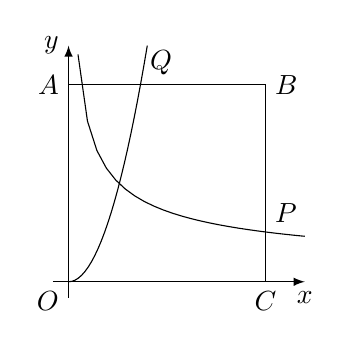
\begin{tikzpicture}[>=latex]
\draw [->] (-0.2,0) -- (3,0) node [below] {$x$};
\draw [->] (0,-0.2) -- (0,3) node [left] {$y$};
\draw (0,0) node [below left] {$O$};
\draw (2.5,0) node [below] {$C$} coordinate (C);
\draw (2.5,2.5) node [right] {$B$} coordinate (B);
\draw (0,2.5) node [left] {$A$} coordinate (A);
\draw [domain = 0:1] plot (\x,{3*\x*\x});
\draw [domain = 0.12:3] plot (\x,{pow(\x,-1/2)});
\draw (C) -- (B) -- (A);
\draw ({sqrt(2.5/3)},2.5) node [above right] {$Q$};
\draw (2.5,{pow(2.5,-1/2)}) node [above right] {$P$};
\end{tikzpicture}
\end{center}


关联目标:

暂未关联目标



标签: 第二单元

答案: 暂无答案

解答或提示: 暂无解答与提示

使用记录:

20211228	2022届高三1班	\fcolorbox[rgb]{0,0,0}{1.000,0.228,0}{0.886}


出处: 2022届高三上学期测验卷11第10题
\item { (004486)}某温室大棚规定: 一天中, 从中午$12$点到第二天上午$8$点为保温时段, 其余$4$小时为工人作业时段. 从中午$12$点连续测量$20$小时, 得出此温室大棚的温度$y$(单位: 度)与时间$t$(单位: 小时, $t\in [0,20]$)近似地满足函数$y=|t-13|+\dfrac b{t+2}$关系, 其中, $b$为大棚内一天中保温时段的通风量.\\
(1) 若一天中保温时段的通风量保持$100$个单位不变, 求大棚一天中保温时段的最低温度(精确到$0.1^\circ\text{C}$);\\
(2) 若要保持大棚一天中保温时段的最低温度不小于$17^\circ\text{C}$, 求大棚一天中保温时段通风量的最小值.


关联目标:

暂未关联目标



标签: 第二单元

答案: 暂无答案

解答或提示: 暂无解答与提示

使用记录:

20211116	2022届高三1班	\fcolorbox[rgb]{0,0,0}{1.000,0.078,0}{0.961}	\fcolorbox[rgb]{0,0,0}{1.000,0.180,0}{0.910}


出处: 2022届高三上学期测验卷07第19题
\item { (004500)}对于定义域为$D$的函数$f(x)$, 若存在$x_1,x_2\in D$且$x_1\ne x_2$, 使得$f(x_1^2)=f(x_2^2)=2f(x_1+x_2)$, 则称函数$f(x)$具有性质$M$. 若函数$g(x)=|\log_2x-1|$, $x\in (0,a]$具有性质$M$, 则实数$a$的最小值为\blank{50}.


关联目标:

暂未关联目标



标签: 第二单元

答案: 暂无答案

解答或提示: 暂无解答与提示

使用记录:

20211123	2022届高三1班	\fcolorbox[rgb]{0,0,0}{0.286,1.000,0}{0.143}


出处: 2022届高三上学期测验卷08第12题
\item { (004525)}已知函数$f(x)=\begin{cases} x^2, & x\text{为无理数}, \\ x, &x\text{为有理数},   \end{cases}$ 则以下$4$个命题:
\textcircled{1} $f(x)$是偶函数; \textcircled{2} $f(x)$在$[0,+\infty)$上是增函数; \textcircled{3} $f(x)$的值域为$\mathbf{R}$; \textcircled{4} 对于任意的正有理数$a$, $g(x)=f(x)-a$存在奇数个零点.
其中正确命题的个数为\bracket{20}.
\fourch{$0$}{$1$}{$2$}{$3$}


关联目标:

暂未关联目标



标签: 第二单元

答案: 暂无答案

解答或提示: 暂无解答与提示

使用记录:

20211129	2022届高三1班	\fcolorbox[rgb]{0,0,0}{1.000,0.326,0}{0.837}


出处: 2022届高三上学期测验卷09第16题
\item { (004542)}已知$p$是实数, 函数$f(x)=10^x$. 若存在实数$m,n$, 使得$f(m+n)=f(m)+f(n)$与$f(m+n+p)=f(m)+f(n)+f(p)$均成立, 则$p$的最大值等于\blank{50}.


关联目标:

暂未关联目标



标签: 第二单元

答案: 暂无答案

解答或提示: 暂无解答与提示

使用记录:

20211214	2022届高三1班	\fcolorbox[rgb]{0,0,0}{0.930,1.000,0}{0.465}


出处: 2022届高三上学期测验卷10第12题
\item { (004544)}设函数$f(x)=\begin{cases}1, & x\in \mathbf{Q}, \\ \pi, &x\not\in \mathbf{Q}.\end{cases}$ 下列结论不正确的是\bracket{20}.
\twoch{$f(x)$是偶函数}{$f(x)$是周期函数}{该函数有最大值也有最小值}{方程$f(f(x))=1$的解集为$\{1\}$}


关联目标:

暂未关联目标



标签: 第二单元

答案: 暂无答案

解答或提示: 暂无解答与提示

使用记录:

20211214	2022届高三1班	\fcolorbox[rgb]{0,0,0}{1.000,0.140,0}{0.930}


出处: 2022届高三上学期测验卷10第14题
\item { (004658)}如图, $A$、$B$、$C$三地有直道相通, $AB=5$千米, $AC=3$千米, $BC=4$千米, 现甲、乙两警员同时从$A$地出发匀速前往$B$地, 经过$t$小时, 他们之间的距离为$f(t)$(单位: 千米), 甲的路线是$AB$, 速度为$5$千米/小时, 乙的路线是$ACB$, 速度为$8$千米/小时, 乙到$B$地后在原地等待, 设$t=t_1$时乙到达$C$地.
\begin{center}
    \begin{tikzpicture}[scale = 0.6]
        \draw (0,0) node [left] {$C$} -- (4,0) node [right] {$B$} -- (0,3) node [above] {$A$} -- cycle;
    \end{tikzpicture}
\end{center}
(1) 求$t_1$及$f(t_1)$的值;\\
(2) 已知警员的对讲机的有效通话距离是$3$千米, 当$t_1\le t\le 1$时, 求$f(t)$的表达式, 并判断$f(t)$在$[t_1,1]$上的最大值是否超过$3$? 说明理由.


关联目标:

暂未关联目标



标签: 第二单元

答案: 暂无答案

解答或提示: 暂无解答与提示

使用记录:

20211209	2022届高三1班	\fcolorbox[rgb]{0,0,0}{1.000,0.106,0}{0.947}	\fcolorbox[rgb]{0,0,0}{1.000,0.454,0}{0.773}

20211209	2022届高三	\fcolorbox[rgb]{0,0,0}{1.000,0.300,0}{0.850}	\fcolorbox[rgb]{0,0,0}{1.000,0.832,0}{0.584}


出处: 2022届高三上月考卷02第19题
\item { (004667)}若函数$f(x)=\sqrt{2x+1}$的反函数为$g(x)$, 则函数$g(x)$的零点为\blank{50}.


关联目标:

暂未关联目标



标签: 第二单元

答案: 暂无答案

解答或提示: 暂无解答与提示

使用记录:

20211109	2022届高三	\fcolorbox[rgb]{0,0,0}{1.000,0.458,0}{0.771}


出处: 2022届高三上期中区统考第7题
\item { (004679)}为实现``碳达峰'', 减少污染, 某化工企业开发了一个废料回收项目. 经测算, 该项目日回收成本$p$(元)与日回收量$x$(吨)($x\in [0,50]$)的函数关系可表示为$p=\begin{cases}20x, & 0\le x\le 30,  \\ x^2+16x-780, & 30<x \le 50,  \end{cases}$ 且每回收$1$吨废料, 转化成其他产品可收入$80$元.\\
(1) 设日纯收益为$y$元, 写出函数$y=f(x)$的解析式(纯收益$=$收入$-$成本);\\
(2) 该公司每日回收废料多少吨时, 获得纯收益最大?


关联目标:

暂未关联目标



标签: 第二单元

答案: 暂无答案

解答或提示: 暂无解答与提示

使用记录:

20211109	2022届高三	\fcolorbox[rgb]{0,0,0}{1.000,0.050,0}{0.975}	\fcolorbox[rgb]{0,0,0}{1.000,0.168,0}{0.916}


出处: 2022届高三上期中区统考第19题
\item { (004680)}已知函数$f(x)=2^x+\dfrac a{2^x}$, $a$为实常数.\\
(1) 若函数$f(x)$为奇函数, 求$a$的值;\\
(2) 若$x\in [0,1]$时$f(x)$的最小值为$2$, 求$a$的值;\\
(3) 若方程$f(x)=6$有两个不等的实根$x_1,x_2$, 且$|x_1-x_2|\le 1$, 求$a$的取值范围.


关联目标:

暂未关联目标



标签: 第二单元

答案: 暂无答案

解答或提示: 暂无解答与提示

使用记录:

20211109	2022届高三	\fcolorbox[rgb]{0,0,0}{1.000,0.234,0}{0.883}	\fcolorbox[rgb]{0,0,0}{1.000,0.340,0}{0.830}	\fcolorbox[rgb]{0,0,0}{1.000,0.906,0}{0.547}


出处: 2022届高三上期中区统考第20题
\item { (004702)}给定区间$I$和正常数$a$, 如果定义在$\mathbf{R}$上的两个函数$y=f(x)$与$y=g(x)$满足: 对一切$x\in I$, 均有$|f(x)-g(x)|\le a$, 称函数$y=f(x)$与$y=g(x)$具有性质$P(I,a)$.\\
(1)	已知$I=(0,+\infty)$, 判断下列两组函数是否具有性质$P(I,2)$? \textcircled{1} $f_1(x)=\dfrac 1{{x^2}+1}$, $g_1(x)=2$; \textcircled{2} $f_2(x)=x^2+x+1$, $g_2(x)=x^2-x+1$;(不需要说明理由)\\
(2)	已知$f(x)=0$, $y=g(x)$是周期函数, 且对任意的$a>0$, 均存在区间$I=(M,+\infty)$, 使得函数$y=f(x)$与$y=g(x)$具有性质$P(I,a)$, 求证: $g(x)=0$;\\
(3)	已知$I=[1,m]$, $f(x)=x^2$, 若存在一次函数$y=g(x)$与$y=f(x)$具有性质$P(I,1)$, 求实数$m$的最大值.


关联目标:

暂未关联目标



标签: 第二单元

答案: 暂无答案

解答或提示: 暂无解答与提示

使用记录:

20211221	2022届高三	\fcolorbox[rgb]{0,0,0}{1.000,0.026,0}{0.987}	\fcolorbox[rgb]{0,0,0}{0.398,1.000,0}{0.199}	\fcolorbox[rgb]{0,0,0}{0.062,1.000,0}{0.031}


出处: 2022届高三上一模第21题
\item { (004720)}已知函数$f(x)=x^2+mx+3$, 其中$m\in \mathbf{R}$.\\
(1) 若不等式$f(x)<5$的解集是$(-1,2)$, 求$m$的值;\\
(2) 若函数$y=f(x)$在区间$[0,3]$上有且仅有一个零点, 求$m$的取值范围.


关联目标:

暂未关联目标



标签: 第二单元

答案: 暂无答案

解答或提示: 暂无解答与提示

使用记录:

20220414	2022届高三	\fcolorbox[rgb]{0,0,0}{1.000,0.042,0}{0.979}	\fcolorbox[rgb]{0,0,0}{1.000,0.670,0}{0.665}


出处: 2022届高三下期中区统考第18题
\item { (004721)}如图, 有一块扇形草地$OMN$, 已知半径为$4$, $\angle MON=\dfrac\pi 2$, 现要在其中圈出一块举行场地$ABCD$作为儿童乐园使用, 其中点$A$、$B$在弧$\overset\frown{MN}$上, 且线段$AB$平行于线段$MN$.
\begin{center}
    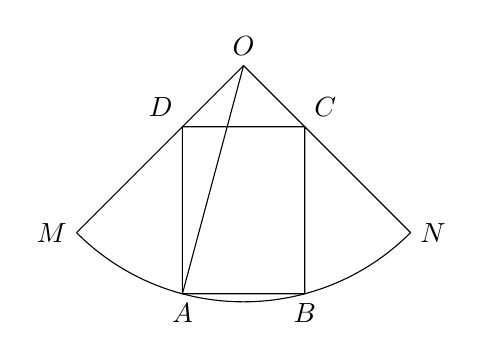
\begin{tikzpicture}[scale = 1.5]
        \draw (0,0) node [above] {$O$} coordinate (O);
        \draw (-45:2) node [right] {$N$} coordinate (N);
        \draw (-135:2) node [left] {$M$} coordinate (M);
        \draw (-75:2) node [below] {$B$} coordinate (B);
        \draw (-105:2) node [below] {$A$} coordinate (A);
        \draw (-45:{2/sin(45)*sin(15)}) node [above right] {$C$} coordinate (C);
        \draw (-135:{2/sin(45)*sin(15)}) node [above left] {$D$} coordinate (D);
        \draw (M) -- (O) -- (N) (A) rectangle (C) (O) -- (A);
        \draw (M) arc (-135:-45:2);
    \end{tikzpicture}
\end{center}
(1) 若点$A$为弧$\overset\frown{MN}$的一个三等分点, 求矩形$ABCD$的面积$S$;\\
(2) 当$A$在何处时, 矩形$ABCD$的面积$S$最大? 最大值为多少?


关联目标:

暂未关联目标



标签: 第二单元

答案: 暂无答案

解答或提示: 暂无解答与提示

使用记录:

20220414	2022届高三	\fcolorbox[rgb]{0,0,0}{1.000,0.302,0}{0.849}	\fcolorbox[rgb]{0,0,0}{1.000,0.652,0}{0.674}


出处: 2022届高三下期中区统考第19题
\item { (004755)}设$y=f^{-1}(x)$是函数$f(x)=\dfrac x2+\dfrac{\pi}8\sin x+\dfrac{\pi}8$, $x\in [-\dfrac{\pi }2,\dfrac{\pi }2]$的反函数, 则函数$y=f(x)+f^{-1}(x)$的最小值等于\blank{50}.


关联目标:

暂未关联目标



标签: 第二单元|第三单元

答案: 暂无答案

解答或提示: 暂无解答与提示

使用记录:

20220317	2022届高三1班	\fcolorbox[rgb]{0,0,0}{1.000,0.884,0}{0.558}


出处: 2022届高三下月考卷01第11题
\item { (004756)}函数$f(x)=x$, $g(x)=x^2-x+2$. 若存在$x_1, x_2,\cdots,x_n\in [0,\dfrac 92]$, 使得$f(x_1)+f(x_2)+...+f(x_{n-1})+g(x_n)=g(x_1)+g(x_2)+...+g(x_{n-1})+f(x_n)$, 则$n$的最大值为\blank{50}.


关联目标:

暂未关联目标



标签: 第二单元

答案: 暂无答案

解答或提示: 暂无解答与提示

使用记录:

20220317	2022届高三1班	\fcolorbox[rgb]{0,0,0}{1.000,0.744,0}{0.628}


出处: 2022届高三下月考卷01第12题
\item { (004995)}从半径为$R$的圆形铁片里剪去一个扇形, 然后把剩下部分卷成一个圆锥形漏斗, 要使漏斗有最大容量, 剪去扇形的圆心角$\theta$应是多少弧度?


关联目标:

K0119001B|D01003B|会运用平均值不等式求解较简单的最大值和最小值问题.



标签: 第一单元|第二单元

答案: 暂无答案

解答或提示: 暂无解答与提示

使用记录:

暂无使用记录


出处: 代数精编第二章不等式
\item { (005012)}若$a>1$, $b>1$, $c>1$, 则$\log_ab+\log_ba$的最小值为\blank{50}, $\log_ab+\log_bc+\log_ca$的最小值为\blank{50}.


关联目标:

K0119001B|D01003B|会运用平均值不等式求解较简单的最大值和最小值问题.



标签: 第一单元|第二单元

答案: 暂无答案

解答或提示: 暂无解答与提示

使用记录:

暂无使用记录


出处: 代数精编第二章不等式
\item { (005014)}若$a>1$, $0<b<1$, 则$\log_ab+\log_ba$的最大值为\blank{50}.


关联目标:

K0206002B|D02001B|会运用对数的运算性质以及换底公式解决较复杂的求值、化简以及证明等相关问题.



标签: 第一单元|第二单元

答案: 暂无答案

解答或提示: 暂无解答与提示

使用记录:

暂无使用记录


出处: 代数精编第二章不等式
\item { (005103)}下列函数中, 最小值为$2$的是\bracket{20}.
\twoch{$x+\dfrac 1x$}{$\dfrac{x^2+2}{\sqrt{x^2+1}}$}{$\log_ax+\log_xa$($a>0$, $x>0$, $a\ne 1$, $x\ne 1$)}{$3^x+3^{-x}$($x>0$)}


关联目标:

K0118002B|D01003B|经历平均值不等式的证明过程, 理解取等号的条件.

K0119001B|D01003B|会运用平均值不等式求解较简单的最大值和最小值问题.

K0206002B|D02001B|会运用对数的运算性质以及换底公式解决较复杂的求值、化简以及证明等相关问题.



标签: 第一单元|第二单元

答案: 暂无答案

解答或提示: 暂无解答与提示

使用记录:

暂无使用记录


出处: 代数精编第二章不等式
\item { (005104)}若$\log_{\sqrt 2}x+\log_{\sqrt 2}y=4$, 则$x+y$的最小值是\bracket{20}.
\fourch{$8$}{$4\sqrt 2$}{$4$}{$2$}


关联目标:

K0205002B|D02001B|会运用对数的定义以及运算性质解决简单的求值、化简以及生活实际问题.

K0119001B|D01003B|会运用平均值不等式求解较简单的最大值和最小值问题.



标签: 第一单元|第二单元

答案: 暂无答案

解答或提示: 暂无解答与提示

使用记录:

暂无使用记录


出处: 代数精编第二章不等式
\item { (005105)}若$a,b$均为大于$1$的正数, 且$ab=100$, 则$\lg a\cdot \lg b$的最大值是\bracket{20}.
\fourch{$0$}{$1$}{$2$}{$\dfrac 52$}


关联目标:

K0119001B|D01003B|会运用平均值不等式求解较简单的最大值和最小值问题.

K0205002B|D02001B|会运用对数的定义以及运算性质解决简单的求值、化简以及生活实际问题.



标签: 第一单元|第二单元

答案: 暂无答案

解答或提示: 暂无解答与提示

使用记录:

暂无使用记录


出处: 代数精编第二章不等式
\item { (005110)}若$x+2y=2\sqrt 2a$($x>0$, $y>0$, $a>1$), 则$\log_ax+\log_ay$的最大值是\blank{50}.


关联目标:

K0119001B|D01003B|会运用平均值不等式求解较简单的最大值和最小值问题.

K0205002B|D02001B|会运用对数的定义以及运算性质解决简单的求值、化简以及生活实际问题.



标签: 第一单元|第二单元

答案: 暂无答案

解答或提示: 暂无解答与提示

使用记录:

暂无使用记录


出处: 代数精编第二章不等式
\item { (005118)}若正数$x,y,z$满足$5x+2y+z=100$, 则$\lg x+\lg y+\lg z$的最大值是\blank{50}.


关联目标:

该题的考查目标不在目前的集合中



标签: 第一单元|第二单元

答案: 暂无答案

解答或提示: 暂无解答与提示

使用记录:

暂无使用记录


出处: 代数精编第二章不等式
\item { (005124)}求函数$y=\dfrac{x^4+3x^2+3}{x^2+1}$的最小值.


关联目标:

暂未关联目标



标签: 第二单元

答案: 暂无答案

解答或提示: 暂无解答与提示

使用记录:

暂无使用记录


出处: 代数精编第二章不等式
\item { (005125)}求$f(x)=4x^2+\dfrac{16}{(x^2+1)^2}$的最小值.


关联目标:

暂未关联目标



标签: 第二单元

答案: 暂无答案

解答或提示: 暂无解答与提示

使用记录:

暂无使用记录


出处: 代数精编第二章不等式
\item { (005126)}求$f(x)=x^2-3x-2-\dfrac 3x+\dfrac 1{x^2}$($x>0$)的最小值.


关联目标:

暂未关联目标



标签: 第二单元

答案: 暂无答案

解答或提示: 暂无解答与提示

使用记录:

暂无使用记录


出处: 代数精编第二章不等式
\item { (005132)}已知函数$f(x)=\dfrac{2^{x+3}}{{4^x}+8}$.\\
(1) 求$f(x)$的最大值;\\
(2) 对于任意实数$a,b$, 求证: $f(a)<b^2-4b+\dfrac{11}2$.


关联目标:

K0119001B|D01003B|会运用平均值不等式求解较简单的最大值和最小值问题.



标签: 第一单元|第二单元

答案: 暂无答案

解答或提示: 暂无解答与提示

使用记录:

暂无使用记录


出处: 代数精编第二章不等式
\item { (005136)}在$\triangle ABC$中, 已知$BC=a$, $CA=b$, $AB=c$, $\angle ACB=\theta$. 现将$\triangle ABC$分别以$BC,CA,AB$所在直线为轴旋转一周, 设所得三个旋转体的体积依次为$V_1,V_2,V_3$.\\
(1) 设$T=\dfrac{V_3}{V_1+V_2}$, 试用$a,b,c$表示$T$;\\
(2) 若$\theta$为定值, 并令$\dfrac{a+b}c=x$, 将$T=\dfrac{V_3}{V_1+V_2}$表示为$x$的函数, 写出这个函数的定义域, 并求这个函数的最大值$M$;\\
(3) 若$\theta \in [\dfrac{\pi }3,\pi)$, 求(2)中$M$的最大值.


关联目标:

K0119002B|D01003B|会运用平均值不等式解决一些现实情境中的最大值和最小值问题.



标签: 第一单元|第二单元

答案: 暂无答案

解答或提示: 暂无解答与提示

使用记录:

暂无使用记录


出处: 代数精编第二章不等式
\item { (005218)}已知$x$满足不等式$(\dfrac 12)^{2x-4}-(\dfrac 12)^x-(\dfrac 12)^{x-2}+\dfrac 14\le 0$, 且$y=\log_{\frac 1a}(a^2x)\cdot \log_{\frac 1{a^2}}(ax)$的最大值是$0$, 最小值是$-\dfrac 18$, 求实数$a$的值.


关联目标:

暂未关联目标



标签: 第二单元

答案: 暂无答案

解答或提示: 暂无解答与提示

使用记录:

暂无使用记录


出处: 代数精编第二章不等式
\item { (005243)}求函数$f(x)=|x-\dfrac 12|-|x+\dfrac 12|$的最大值.


关联目标:

暂未关联目标



标签: 第二单元

答案: 暂无答案

解答或提示: 暂无解答与提示

使用记录:

暂无使用记录


出处: 代数精编第二章不等式
\item { (005278)}已知函数$y=f(x)=x^2+ax+3$在区间$x\in [-1,1]$上的最小值为$-3$, 求实数$a$的值.


关联目标:

暂未关联目标



标签: 第二单元

答案: 暂无答案

解答或提示: 暂无解答与提示

使用记录:

暂无使用记录


出处: 代数精编第三章函数
\item { (005332)}若$2x^2-3x\le 0$, 则函数$f(x)=x^2+x+1$\bracket{20}.
\twoch{有最小值$\dfrac 34$, 但无最大值}{有最小值$\dfrac 34$, 有最大值1}{有最小值1有最大值$\dfrac{19}4$}{既无最小值, 也无最大值}


关联目标:

暂未关联目标



标签: 第二单元

答案: 暂无答案

解答或提示: 暂无解答与提示

使用记录:

暂无使用记录


出处: 代数精编第三章函数
\item { (005344)}已知函数$f(x)=x^2-2x+3$在$[0,m]$上有最大值$3$, 最小值$2$, 求正数$m$的取值范围.


关联目标:

暂未关联目标



标签: 第二单元

答案: 暂无答案

解答或提示: 暂无解答与提示

使用记录:

暂无使用记录


出处: 代数精编第三章函数
\item { (005345)}已知函数$y=x^2+mx-1$在区间$[0,3]$上有最小值$-2$, 求实数$m$的值.


关联目标:

暂未关联目标



标签: 第二单元

答案: 暂无答案

解答或提示: 暂无解答与提示

使用记录:

暂无使用记录


出处: 代数精编第三章函数
\item { (005346)}当$x\ge 0$时, 求函数$f(x)=x^2+2ax$的最小值.


关联目标:

暂未关联目标



标签: 第二单元

答案: 暂无答案

解答或提示: 暂无解答与提示

使用记录:

暂无使用记录


出处: 代数精编第三章函数
\item { (005357)}将进货单价为$40$元的商品按每件$50$元出售时, 每月能卖出$500$个, 已知这批商品在销售单价的基础上每涨价$1$元, 其月销售数就减少$10$个, 为了每月赚取最大利润, 销售单价应定为多少?


关联目标:

暂未关联目标



标签: 第二单元

答案: 暂无答案

解答或提示: 暂无解答与提示

使用记录:

暂无使用记录


出处: 代数精编第三章函数
\item { (005358)}飞机飞行$1$小时的耗费由两部分组成: 固定部分$4900$元, 变动部分$P$与飞机飞行速度$v$(千米/时)的函数关系是$P=0.01v^2$. 已知甲、乙两地相距为一常数$a$(千米), 试写出飞机从甲地飞到乙地的总耗费$y$与飞机速度$v$的函数关系式, 并写出耗费最小时飞机的飞行速度.


关联目标:

暂未关联目标



标签: 第二单元

答案: 暂无答案

解答或提示: 暂无解答与提示

使用记录:

暂无使用记录


出处: 代数精编第三章函数
\item { (005499)}若奇函数$f(x)$在区间$[-3, -1]$上是增函数, 且有最大值$-2$, 则$f(x)$在$[1, 3]$上是\blank{50}函数(填``增''或``减''), 且最小值等于\blank{50}.


关联目标:

暂未关联目标



标签: 第二单元

答案: 暂无答案

解答或提示: 暂无解答与提示

使用记录:

暂无使用记录


出处: 代数精编第三章函数
\item { (005531)}已知函数$y=-\sqrt {1-x^2}$的反函数是$y=-\sqrt {1-x^2}$, 则原函数的定义域``最大''可以是\blank{50}.


关联目标:

暂未关联目标



标签: 第二单元

答案: 暂无答案

解答或提示: 暂无解答与提示

使用记录:

暂无使用记录


出处: 代数精编第三章函数
\item { (005560)}求函数$y=9^x-m\cdot 3^x+1$的最小值.


关联目标:

暂未关联目标



标签: 第二单元

答案: 暂无答案

解答或提示: 令$t=3^x$则函数为$y=t^2-mt+1=(t-\dfrac m2)^2+1-\dfrac{m^2}4$, 其图像的对称轴方程为$t=\dfrac m2$.
(1) 如下图左, 若$\dfrac m2>0$, 则当$t=\dfrac m2$时, $y_{\min }=1-\dfrac{m^2}4$.
\begin{center}
    \begin{tikzpicture}[>=latex]
        \draw [->] (-1,0) -- (3,0) node [below] {$t$};
        \draw [->] (0,-1) -- (0,3) node [left] {$y$};
        \draw (0,0) node [below left] {$O$};
        \draw [dashed, domain = -0.5:0, samples = 100] plot (\x,{(\x-1)^2/2+1});
        \draw [domain = 0:2.5, samples = 100] plot (\x,{(\x-1)^2/2+1});
        \draw [dashed] (1,-0.5) -- (1,2.5);
        \draw (1,0) node [below right] {$\frac{m}{2}$};
        \filldraw [white] (0,1.5) circle (0.05);
        \draw (0,1.5) circle (0.05);
    \end{tikzpicture}
    \begin{tikzpicture}[>=latex]
        \draw [->] (-3,0) -- (1,0) node [below] {$t$};
        \draw [->] (0,-1) -- (0,3) node [left] {$y$};
        \draw (0,0) node [below left] {$O$};
        \draw [dashed, domain = -2.5:0, samples = 100] plot (\x,{(\x+1)^2/2+1});
        \draw [domain = 0:0.5, samples = 100] plot (\x,{(\x+1)^2/2+1});
        \draw [dashed] (-1,-0.5) -- (-1,2.5);
        \draw (-1,0) node [below right] {$\frac{m}{2}$};
        \filldraw [white] (0,1.5) circle (0.05);
        \draw (0,1.5) circle (0.05);
    \end{tikzpicture}
\end{center}
(2) 如上图右, 若$\dfrac m2\le 0$, 则由于$t>0$, 函数无最小值.

使用记录:

暂无使用记录


出处: 代数精编第三章函数
\item { (005585)}若$1\le x\le 2$, 则函数$y=(\dfrac 12)^{x^2-6x+10}$的最大值为\blank{50}.


关联目标:

暂未关联目标



标签: 第二单元

答案: 暂无答案

解答或提示: 暂无解答与提示

使用记录:

暂无使用记录


出处: 代数精编第三章函数
\item { (005586)}函数$f(x)=a^{2x}-3a^x+2$($a>0$且$a\ne 1$)的最小值为\blank{50}.


关联目标:

暂未关联目标



标签: 第二单元

答案: 暂无答案

解答或提示: 暂无解答与提示

使用记录:

暂无使用记录


出处: 代数精编第三章函数
\item { (005587)}对于函数$y=a^{x^2-4}$($a>0$且$a\ne 1$):\\
(1) 若$0<a<1$, 则$y$有最大值\blank{50};\\
(2) 若$a>1$, 则$y$有最小值\blank{50}.


关联目标:

暂未关联目标



标签: 第二单元

答案: 暂无答案

解答或提示: 暂无解答与提示

使用记录:

暂无使用记录


出处: 代数精编第三章函数
\item { (005598)}若$0\le x\le 2$, 求函数$y=4^{x-\frac 12}-3\cdot 2^x+5$的最大值和最小值.


关联目标:

暂未关联目标



标签: 第二单元

答案: 暂无答案

解答或提示: 暂无解答与提示

使用记录:

暂无使用记录


出处: 代数精编第三章函数
\item { (005599)}若函数$f(x)=a^{2x}+2a^x-1$($a>0$且$a\ne 1$)在$[-1, 1]$上的最大值为$14$, 求实数$a$的值.


关联目标:

暂未关联目标



标签: 第二单元

答案: 暂无答案

解答或提示: 暂无解答与提示

使用记录:

暂无使用记录


出处: 代数精编第三章函数
\item { (005644)}已知函数$f(x)=x^2\lg a+2x+4\lg a$的最大值为3, 求实数$a$的值.


关联目标:

暂未关联目标



标签: 第二单元

答案: 暂无答案

解答或提示: 暂无解答与提示

使用记录:

暂无使用记录


出处: 代数精编第三章函数
\item { (005733)}若$-3\le \log_{\frac 12}x\le -\dfrac 12$, 求$y=(\log_2\dfrac x2)(\log_2\dfrac x4)$的最大(小)值及其相应的$x$值,


关联目标:

暂未关联目标



标签: 第二单元

答案: 暂无答案

解答或提示: 暂无解答与提示

使用记录:

暂无使用记录


出处: 代数精编第三章函数
\item { (005734)}已知$a,b$是两个不相等的正数, 且$\log_m\dfrac xa\cdot \log_m\dfrac xb$的最小值是$-\dfrac 14$($m>0$且$m\ne 1$), 求$m$的值.


关联目标:

暂未关联目标



标签: 第二单元

答案: 暂无答案

解答或提示: 暂无解答与提示

使用记录:

暂无使用记录


出处: 代数精编第三章函数
\item { (005735)}已知实数$x,y$满足$(\log_4y)^2=\log_{\frac 12}x$, 求$u=\dfrac xy$的最大值及其相应的$x,y$的值.


关联目标:

暂未关联目标



标签: 第二单元

答案: 暂无答案

解答或提示: 暂无解答与提示

使用记录:

暂无使用记录


出处: 代数精编第三章函数
\item { (005740)}若二次函数$f(x)=(\lg a)x^2+2x+4\lg a$有最小值$-3$, 求实数$a$的值.


关联目标:

暂未关联目标



标签: 第二单元

答案: 暂无答案

解答或提示: 暂无解答与提示

使用记录:

暂无使用记录


出处: 代数精编第三章函数
\item { (005751)}已知函数$f(x)=\lg \dfrac{x+1}{x-1}+\lg (x-1)+\lg (a-x)$($a>1$).\\
(1) 是否存在一个实数$a$使得函数$y=f(x)$的图像关于某一条垂直于$x$轴的直线对称? 若存在, 求出这个实数$a$; 若不存在, 说明理由;\\
(2) 当$f(x)$的最大值为2时, 求实数$a$的值.


关联目标:

暂未关联目标



标签: 第二单元

答案: 暂无答案

解答或提示: 暂无解答与提示

使用记录:

暂无使用记录


出处: 代数精编第三章函数
\item { (005812)}已知函数$f(x)=x^2\lg a+2x+4\lg a$的最大值是$3$, 求实数$a$的值.


关联目标:

暂未关联目标



标签: 第二单元

答案: 暂无答案

解答或提示: 暂无解答与提示

使用记录:

暂无使用记录


出处: 代数精编第三章函数
\item { (005834)}(1)求函数$y=2x+\sqrt {1-2x}$的最大值.
(2)求函数$y=2x+\sqrt {1-x^2}$的值域.
(3)求函数$y=\dfrac{\sqrt {x+1}}{x+2}$的值域.


关联目标:

暂未关联目标



标签: 第二单元

答案: 暂无答案

解答或提示: 暂无解答与提示

使用记录:

暂无使用记录


出处: 代数精编第三章函数
\item { (005838)}已知函数$f(x)=x^2-2mx+m+6$.\\
(1) 若对任意实数$x$都有$f(x)>0$, 求实数$m$的取值范围;\\
(2) 若实数$\alpha ,\beta$满足$f(\alpha)=f(\beta)=0$, 求$\alpha ^2+\beta ^2$的最小值.


关联目标:

暂未关联目标



标签: 第二单元

答案: 暂无答案

解答或提示: 暂无解答与提示

使用记录:

暂无使用记录


出处: 代数精编第三章函数
\item { (005840)}已知$f(x)=-9x^2-6ax+2a-a^2$在$-\dfrac 13\le x\le \dfrac 13$内有最大值$-3$, 求实数$a$的值.


关联目标:

暂未关联目标



标签: 第二单元

答案: 暂无答案

解答或提示: 暂无解答与提示

使用记录:

暂无使用记录


出处: 代数精编第三章函数
\item { (005850)}已知函数$f(x)=\log_3(x^2-4mx+4m^2+m+\dfrac 1{m-1})$, 集合$M=\{m|m>1,m\in \mathbf{R}\}$.\\
(1) 求证: 当$m\in M$时, $f(x)$的定义域为$x\in \mathbf{R}$; 反之, 若$f(x)$对一切实数$x$都有意义, 则$m\in M$;\\
(2) 当$m\in M$时, 求$f(x)$的最小值;\\
(3) 求证: 对每一个$m\in M$, $f(x)$的最小值都不小于1.


关联目标:

暂未关联目标



标签: 第二单元

答案: 暂无答案

解答或提示: 暂无解答与提示

使用记录:

暂无使用记录


出处: 代数精编第三章函数
\item { (007904)}求函数$f(x)=x^2-4x-2$的最小值, 并求出取最值时相应的自变量$x$的值.


关联目标:

暂未关联目标



标签: 第二单元

答案: 暂无答案

解答或提示: 暂无解答与提示

使用记录:

暂无使用记录


出处: 二期课改练习册高一第一学期
\item { (007905)}求函数$f(x)=6x-3x^2$的最小值, 并求出取最值时相应的自变量$x$的值.


关联目标:

暂未关联目标



标签: 第二单元

答案: 暂无答案

解答或提示: 暂无解答与提示

使用记录:

暂无使用记录


出处: 二期课改练习册高一第一学期
\item { (007906)}求函数$f(x)=-x^2-4x-3,x\in [-3,1]$的最小值, 并求出取最值时相应的自变量$x$的值.


关联目标:

暂未关联目标



标签: 第二单元

答案: 暂无答案

解答或提示: 暂无解答与提示

使用记录:

暂无使用记录


出处: 二期课改练习册高一第一学期
\item { (007907)}求函数$f(x)=x^2-2x-3,x\in [-2,0]$的最小值, 并求出取最值时相应的自变量$x$的值.


关联目标:

暂未关联目标



标签: 第二单元

答案: 暂无答案

解答或提示: 暂无解答与提示

使用记录:

暂无使用记录


出处: 二期课改练习册高一第一学期
\item { (007908)}已知$p$、$q$分别是函数$f(x)=-2x+3$在$[-2,2]$上的最大值和最小值, 求函数$g(x)=2x^2-px+q$在$[-2,2]$上的最大值和最小值.


关联目标:

暂未关联目标



标签: 第二单元

答案: 暂无答案

解答或提示: 暂无解答与提示

使用记录:

暂无使用记录


出处: 二期课改练习册高一第一学期
\item { (007909)}求函数$y=\dfrac 2{x-1}(2\le x\le 6)$的最大值与最小值.


关联目标:

暂未关联目标



标签: 第二单元

答案: 暂无答案

解答或提示: 暂无解答与提示

使用记录:

暂无使用记录


出处: 二期课改练习册高一第一学期
\item { (007910)}求函数$f(x)=x^3+x^2+x-1$在区间$(0,1)$内的零点(精确到$0.1$).


关联目标:

暂未关联目标



标签: 第二单元

答案: 暂无答案

解答或提示: 暂无解答与提示

使用记录:

暂无使用记录


出处: 二期课改练习册高一第一学期
\item { (007911)}画出函数$y=x^2-2|x|$的图像, 并写出它的定义域、奇偶性、单调区间、最小值.


关联目标:

暂未关联目标



标签: 第二单元

答案: 暂无答案

解答或提示: 暂无解答与提示

使用记录:

暂无使用记录


出处: 二期课改练习册高一第一学期
\item { (007912)}研究函数$f(x)=\dfrac 1{1+x^2}$的定义域、奇偶性、单调性、最大值.


关联目标:

暂未关联目标



标签: 第二单元

答案: 暂无答案

解答或提示: 暂无解答与提示

使用记录:

暂无使用记录


出处: 二期课改练习册高一第一学期
\item { (007917)}已知$\alpha,\beta$是方程$4x^2-4mx+m+2=0$的两个实数根, 当$m$为何值时, $\alpha ^2+\beta ^2$有最小值? 并求出这个最小值.


关联目标:

暂未关联目标



标签: 第二单元

答案: 暂无答案

解答或提示: 暂无解答与提示

使用记录:

暂无使用记录


出处: 二期课改练习册高一第一学期
\item { (007918)}求函数$y=x^2-4x+1$在$x\in [t,4]$上的最小值和最大值, 其中$t<4$.


关联目标:

暂未关联目标



标签: 第二单元

答案: 暂无答案

解答或提示: 暂无解答与提示

使用记录:

暂无使用记录


出处: 二期课改练习册高一第一学期
\item { (007919)}已知集合$A=\{x|1\le x\le 4\}$, $f(x)=x^2+px+q$和$g(x)=x+\dfrac 4x$是定义在$A$上的函数, 且在$x_0$处同时取到最小值, 并满足$f(x_0)=g(x_0)$, 求$f(x)$在$A$上的最大值.


关联目标:

暂未关联目标



标签: 第二单元

答案: 暂无答案

解答或提示: 暂无解答与提示

使用记录:

暂无使用记录


出处: 二期课改练习册高一第一学期
\item { (007920)}已知某气垫船的最大船速是$48$海里/时, 船每小时使用的燃料费用和船速的平方成正比, 若船速为$30$海里/时, 则船每小时的燃料费用为$600$元.其余费用(不论船速为多少)都是每小时$864$元.甲乙两地相距$100$海里, 船从甲地行驶到乙地.\\
(1) 试把船每小时使用的燃料费用$P$(元)表示成船速$v$(海里/时)的函数;\\
(2) 试把船从甲地到乙地所需的总费用$y$表示成船速$v$(海里/时)的函数;\\
(3) 当船速为每小时多少海里时, 船从甲地到乙地所需的总费用最少?


关联目标:

暂未关联目标



标签: 第二单元

答案: 暂无答案

解答或提示: 暂无解答与提示

使用记录:

暂无使用记录


出处: 二期课改练习册高一第一学期
\item { (007921)}已知函数$y=f(x)$, 定义$F(x)=f(x+1)-f(x)$.某公司每月最多生产$100$台报警系统装置, 生产$x$台$(x>0)$的收入函数为$R(x)=3000x-20x^2$(单位: 元), 其成本函数为$G(x)=5000x+4000$(单位: 元), 利润是收入与成本之差.\\
(1) 求利润函数$y=f(x)$及相应的$y=F(x)$;\\
(2) 利润函数$y=f(x)$与$y=F(x)$是否具有相等的最大值?


关联目标:

暂未关联目标



标签: 第二单元

答案: 暂无答案

解答或提示: 暂无解答与提示

使用记录:

暂无使用记录


出处: 二期课改练习册高一第一学期
\item { (007935)}设$\alpha,\beta$是二次方程$x^2-2kx+k+20=0$的两个实数根, 当$k$为何值时, $(\alpha +1)^2+(\beta +1)^2$有最小值?


关联目标:

暂未关联目标



标签: 第二单元

答案: 暂无答案

解答或提示: 暂无解答与提示

使用记录:

暂无使用记录


出处: 二期课改练习册高一第一学期
\item { (007938)}已知函数$f(x)=-x^2+2ax+1-a$在$[0,1]$上有最大值$2$, 求实数$a$的值.


关联目标:

暂未关联目标



标签: 第二单元

答案: 暂无答案

解答或提示: 暂无解答与提示

使用记录:

暂无使用记录


出处: 二期课改练习册高一第一学期
\item { (007940)}已知函数$f(x)=2-x^2$, 函数$g(x)=x$, 定义函数$F(x)$如下: 当$f(x)\ge g(x)$时, $F(x)=g(x)$; 当$f(x)<g(x)$时, $F(x)=f(x)$. 求$F(x)$的最大值.


关联目标:

暂未关联目标



标签: 第二单元

答案: 暂无答案

解答或提示: 暂无解答与提示

使用记录:

暂无使用记录


出处: 二期课改练习册高一第一学期
\item { (007947)}已知函数$f(x)=x^3-3x$.\\
(1) 试求函数$y=f(x)$的零点;\\
(2) 求证: 函数$f(x)=x^3-3x$在$[1,+\infty)$上是增函数;\\
(3) 是否存在自然数$n$, 使$f(n)=1000$? 若存在, 求出一个满足条件的$n$; 若不存在, 请问明理由.


关联目标:

暂未关联目标



标签: 第二单元

答案: 暂无答案

解答或提示: 暂无解答与提示

使用记录:

暂无使用记录


出处: 二期课改练习册高一第一学期
\item { (007989)}已知函数$f(x)=a^x(a>0,a\ne 1)$在区间$[1,2]$上的最大值比最小值大$\dfrac 14$, 求实数$a$的值.


关联目标:

暂未关联目标



标签: 第二单元

答案: 暂无答案

解答或提示: 暂无解答与提示

使用记录:

暂无使用记录


出处: 二期课改练习册高一第一学期
\item { (007994)}若$2x+y=1$, 求$4^x+2^y$的最小值.


关联目标:

暂未关联目标



标签: 第二单元

答案: 暂无答案

解答或提示: 暂无解答与提示

使用记录:

暂无使用记录


出处: 二期课改练习册高一第一学期
\item { (007998)}甲乙两地的高速公路全长$166$千米, 在高速公路上最高行驶时速不得高于$120$千米/时, 假设汽车从甲地进入该高速公路以不低于$70$千米/时的速度匀速行驶到乙地, 已知汽车每小时的运输成本(以元为单位)由可变部分和固定部分组成: 可变部分与速度$v$(千米/时)的平方成正比, 比例系数为$0.02$; 固定部分为$220$元.\\
(1) 把全程运输成本$y$(元)表示为速度$v$(千米/时)的函数, 并指出这个函数的定义域;\\
(2) 汽车应以多大速度行驶才能使全程运输成本最小? 最小运输成本约为多少元?


关联目标:

暂未关联目标



标签: 第二单元

答案: 暂无答案

解答或提示: 暂无解答与提示

使用记录:

暂无使用记录


出处: 二期课改练习册高一第一学期
\item { (008054)}求函数$y=\log _{\frac 15}(x^2-6x+10)$在区间$[1,2]$上的最大值.


关联目标:

暂未关联目标



标签: 第二单元

答案: 暂无答案

解答或提示: 暂无解答与提示

使用记录:

暂无使用记录


出处: 二期课改练习册高一第二学期
\item { (008086)}已知$\lg x+\lg y=2$, 求$\dfrac 1x+\dfrac 1y$的最小值.


关联目标:

暂未关联目标



标签: 第二单元

答案: 暂无答案

解答或提示: 暂无解答与提示

使用记录:

暂无使用记录


出处: 二期课改练习册高一第二学期
\item { (009497)}已知指数函数$y=a^x$($0<a<1$)在区间$[1, 2]$上的最大值比最小值大$\dfrac a3$, 求实数$a$的值.


关联目标:

暂未关联目标



标签: 第二单元

答案: 暂无答案

解答或提示: 暂无解答与提示

使用记录:

暂无使用记录


出处: 新教材必修第一册课堂练习
\item { (009523)}求函数$y=(\dfrac 12)^x$, $x\in [1, 3]$的最大值与最小值.


关联目标:

暂未关联目标



标签: 第二单元

答案: 暂无答案

解答或提示: 暂无解答与提示

使用记录:

暂无使用记录


出处: 新教材必修第一册课堂练习
\item { (009524)}求下列函数的最大值与最小值:\\
(1) $y=1-x^2$;\\
(2) $y=1-x^2$, $x\in [-1, 2]$;\\
(3) $y=2x^2-8x$;\\
(4) $y=2x^2-8x$, $x\in [0, 1]$.


关联目标:

暂未关联目标



标签: 第二单元

答案: 暂无答案

解答或提示: 暂无解答与提示

使用记录:

暂无使用记录


出处: 新教材必修第一册课堂练习
\item { (009525)}已知$a>-2$, 求函数$y=x^2+1$, $x\in [-2, a]$的最大值.


关联目标:

暂未关联目标



标签: 第二单元

答案: 暂无答案

解答或提示: 暂无解答与提示

使用记录:

暂无使用记录


出处: 新教材必修第一册课堂练习
\item { (009530)}用函数的观点解不等式: $2^x+\log_2x>2$.


关联目标:

暂未关联目标



标签: 第二单元

答案: 暂无答案

解答或提示: 暂无解答与提示

使用记录:

暂无使用记录


出处: 新教材必修第一册课堂练习
\item { (009531)}对于在区间$[a, b]$上的图像是一段连续曲线的函数$y=f(x)$, 如果$f(a)\cdot f(b)>0$, 那么是否该函数在区间$(a, b)$上一定无零点? 说明理由.


关联目标:

暂未关联目标



标签: 第二单元

答案: 暂无答案

解答或提示: 暂无解答与提示

使用记录:

暂无使用记录


出处: 新教材必修第一册课堂练习
\item { (009532)}已知函数$y=2x^3-3x^2-18x+28$在区间$(1, 2)$上有且仅有一个零点. 试用二分法求出该零点的近似值. (结果精确到$0.1$)


关联目标:

暂未关联目标



标签: 第二单元

答案: 暂无答案

解答或提示: 暂无解答与提示

使用记录:

暂无使用记录


出处: 新教材必修第一册课堂练习
\item { (009922)}判断下列说法是否正确, 并说明理由:\\
(1) 函数在某区间上的极大值不会小于它的极小值;\\
(2) 函数在某区间上的最大值不会小于它的最小值;\\
(3) 函数在某区间上的极大值就是它在该区间上的最大值;\\
(4) 函数在某区间上的最大值就是它在该区间上的极大值.


关联目标:

暂未关联目标



标签: 第二单元

答案: 暂无答案

解答或提示: 暂无解答与提示

使用记录:

暂无使用记录


出处: 新教材选择性必修第二册课堂练习
\item { (009924)}求函数$y=x^3-3x$在区间$[-\dfrac 32,0]$上的最大值与最小值.


关联目标:

暂未关联目标



标签: 第二单元

答案: 暂无答案

解答或提示: 暂无解答与提示

使用记录:

暂无使用记录


出处: 新教材选择性必修第二册课堂练习
\item { (009925)}商品的成本$C$和产量$q$满足函数关系$C=50000+200q$, 该商品的销售单价$p$和产量$q$满足函数关系$p=24200-\dfrac 15q^2$. 问: 要使利润最大, 应如何确定产量?


关联目标:

暂未关联目标



标签: 第二单元

答案: 暂无答案

解答或提示: 暂无解答与提示

使用记录:

暂无使用记录


出处: 新教材选择性必修第二册课堂练习
\item { (009926)}采矿、采石或取土时, 常用炸药包进行爆破, 部分爆破呈圆锥漏斗形状(如图), 已知圆锥的母线长是炸药包的爆破半径$R$, 它的值是固定的. 问: 炸药包埋多深可使爆破体积最大? 
\begin{center}
\begin{tikzpicture}[>=latex,scale = 1.6]
\draw (-1,0) -- (1,0) (0.5,0) node [above] {$r$};
\draw (-1,0) -- (0,-2) -- (1,0);
\draw (0,0) ellipse (1 and 0.25);
\draw [dashed] (0,0) -- (0,-2) (0,-1) node [left] {$h$};
\draw (0.5,-1) node [below right] {$R$};
\filldraw (0,-2) circle (0.08) (0,-2.3) node {炸药包};
\end{tikzpicture}
\end{center}


关联目标:

暂未关联目标



标签: 第二单元

答案: 暂无答案

解答或提示: 暂无解答与提示

使用记录:

暂无使用记录


出处: 新教材选择性必修第二册课堂练习
\item { (010147)}已知指数函数$y=a^x$($a>0$且$a\ne 1)$在区间$[1, 2]$上的最大值与最小值之和等于$6$, 求实数$a$的值.


关联目标:

暂未关联目标



标签: 第二单元

答案: 暂无答案

解答或提示: 暂无解答与提示

使用记录:

暂无使用记录


出处: 新教材必修第一册习题
\item { (010161)}已知对数函数$y=\log_ax$($a>1$)在区间$[1, 2]$上的最大值比最小值大$1$, 求$a$的值.


关联目标:

暂未关联目标



标签: 第二单元

答案: 暂无答案

解答或提示: 暂无解答与提示

使用记录:

暂无使用记录


出处: 新教材必修第一册习题
\item { (010179)}求下列函数的最大值与最小值, 并写出取最值时相应自变量的值:\\
(1) $y=x^2-4x-2$;\\
(2) $y=6x-3x^2$;\\
(3) $y=-x^2-4x-3$, $x\in [-3, 1]$;\\
(4) $y=x^2-2x-3$, $x\in [-2, 0]$.


关联目标:

暂未关联目标



标签: 第二单元

答案: 暂无答案

解答或提示: 暂无解答与提示

使用记录:

暂无使用记录


出处: 新教材必修第一册习题
\item { (010180)}求函数$y=\log_{\frac 12}(x+2)$, $x\in [2, 6]$的最大值与最小值.


关联目标:

暂未关联目标



标签: 第二单元

答案: 暂无答案

解答或提示: 暂无解答与提示

使用记录:

暂无使用记录


出处: 新教材必修第一册习题
\item { (010181)}已知$y=x^2+px+q$和$y=x+\dfrac 4x$都是定义在$[1, 4]$上的函数, 且在$x_0$处同时取到相同的最小值. 求$y=x^2+px+q$的最大值.


关联目标:

暂未关联目标



标签: 第二单元

答案: 暂无答案

解答或提示: 暂无解答与提示

使用记录:

暂无使用记录


出处: 新教材必修第一册习题
\item { (010185)}作出函数$y=x^2-2|x|$的大致图像, 并分别写出它的定义域、奇偶性、单调区间及最小值.


关联目标:

暂未关联目标



标签: 第二单元

答案: 暂无答案

解答或提示: 暂无解答与提示

使用记录:

暂无使用记录


出处: 新教材必修第一册习题
\item { (010186)}研究函数$y=\dfrac1{1+x^2}$的定义域、奇偶性、单调性及最大值.


关联目标:

暂未关联目标



标签: 第二单元

答案: 暂无答案

解答或提示: 暂无解答与提示

使用记录:

暂无使用记录


出处: 新教材必修第一册习题
\item { (010188)}设$t$是实数, 且$t<4$. 求函数$y=|2^{x+1}-8|$, $x\in [t, 4]$的最小值.


关联目标:

暂未关联目标



标签: 第二单元

答案: 暂无答案

解答或提示: 暂无解答与提示

使用记录:

暂无使用记录


出处: 新教材必修第一册习题
\item { (010191)}求函数$y=\sqrt{2x+1}-x+1$的零点.


关联目标:

暂未关联目标



标签: 第二单元

答案: 暂无答案

解答或提示: 暂无解答与提示

使用记录:

暂无使用记录


出处: 新教材必修第一册习题
\item { (010192)}已知函数$y=x^3+x^2+x-1$在区间$(0, 1)$上有且仅有一个零点, 用二分法求该零点的近似值. (结果精确到$0.1$)


关联目标:

暂未关联目标



标签: 第二单元

答案: 暂无答案

解答或提示: 暂无解答与提示

使用记录:

暂无使用记录


出处: 新教材必修第一册习题
\item { (010193)}已知某气垫船的最大船速是$48$海里/时, 船每小时使用的燃料费用和船速的平方成正比. 当船速为$30$海里/时时, 船每小时的燃料费用为$600$元, 而其余费用(不论船速为多少)都是每小时$864$元. 船从甲地行驶到乙地, 甲乙两地相距$100$海里.\\
(1) 试把船每小时使用的燃料费用$P$(单位: 元)表示成船速$v$(单位: 海里/时)的函数;\\
(2) 试把船从甲地到乙地所需的总费用$y$(单位:元)表示成船速$v$(单位: 海里/时)的函数;\\
(3) 当船速为多少时, 船从甲地到乙地所需的总费用最少?


关联目标:

暂未关联目标



标签: 第二单元

答案: 暂无答案

解答或提示: 暂无解答与提示

使用记录:

暂无使用记录


出处: 新教材必修第一册习题
\item { (010821)}某函数图像如图所示, 它在$[a, b]$上哪一点处取得最大值? 它是极大值点吗? 在哪一点处取得最小值? 它是极小值点吗? 
\begin{center}
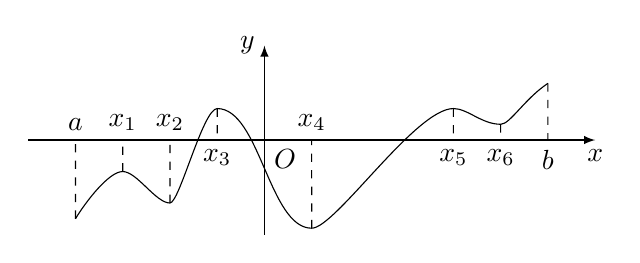
\begin{tikzpicture}[>=latex,xscale = 0.6,yscale = 0.4]
\draw [->] (-5,0) -- (7,0) node [below] {$x$};
\draw [->] (0,-3) -- (0,3) node [left] {$y$};
\draw (0,0) node [below right] {$O$};
\draw (-4,-2.5) coordinate (A) .. controls (-3.8,-2) and (-3.3,-1) .. (-3,-1) coordinate (B) .. controls (-2.7,-1) and (-2.3,-2) .. (-2,-2) coordinate (C) .. controls (-1.8,-2) and (-1.3,1) .. (-1,1) coordinate (D) .. controls (-0.1,1) and (0.1,-2.8) .. (1,-2.8) coordinate (E) .. controls (1.5,-2.8) and (3.2,1) .. (4,1) coordinate (F) .. controls (4.3,1) and (4.6,0.5) .. (5,0.5) coordinate (G) .. controls (5.2,0.5) and (5.5,1.3) .. (6,1.8) coordinate (H);
\draw [dashed] (A) -- (-4,0) node [above] {$a$} (B) -- (-3,0) node [above] {$x_1$} (C) -- (-2,0) node [above] {$x_2$} (D) -- (-1,0) node [below] {$x_3$} (E) -- (1,0) node [above] {$x_4$} (F) -- (4,0) node [below] {$x_5$} (G) -- (5,0) node [below] {$x_6$} (H) -- (6,0) node [below] {$b$};
\end{tikzpicture}
\end{center}


关联目标:

暂未关联目标



标签: 第二单元

答案: 暂无答案

解答或提示: 暂无解答与提示

使用记录:

暂无使用记录


出处: 新教材选择性必修第二册习题
\item { (010829)}用长为$18\text{m}$的钢条制作一个如图所示的长方体框架. 已知长方体的长宽比为$2:1$, 问:该长方体的长、宽、高各为多少时, 其体积最大? 最大体积是多少?
\begin{center}
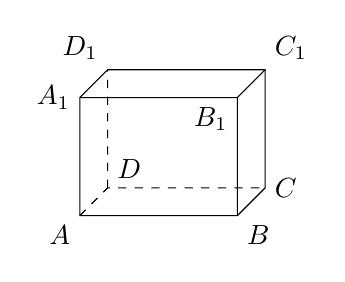
\begin{tikzpicture}[>=latex]
\draw (0,0) node [below left] {$A$} coordinate (A) --++ (2,0) node [below right] {$B$} coordinate (B) --++ (45:{1/2}) node [right] {$C$} coordinate (C)
--++ (0,1.5) node [above right] {$C_1$} coordinate (C1)
--++ (-2,0) node [above left] {$D_1$} coordinate (D1) --++ (225:{1/2}) node [left] {$A_1$} coordinate (A1) -- cycle;
\draw (A) ++ (2,1.5) node [below left] {$B_1$} coordinate (B1) -- (B) (B1) --++ (45:{1/2}) (B1) --++ (-2,0);
\draw [dashed] (A) --++ (45:{1/2}) node [above right] {$D$} coordinate (D) --++ (2,0) (D) --++ (0,1.5);
\end{tikzpicture}
\end{center}


关联目标:

暂未关联目标



标签: 第二单元

答案: 暂无答案

解答或提示: 暂无解答与提示

使用记录:

暂无使用记录


出处: 新教材选择性必修第二册习题
\item { (010830)}某分公司经销一品牌产品, 每件产品的成本为$4$元, 且每件产品需向总公司交$3$元的管理费, 预计当每件产品的售价为$x$元($8\le x\le 11$)时, 一年的销售量为$(12-x)^2$万件. 问:当每件产品的售价为多少元时, 该分公司一年的利润犔最大? (结果精确到$1$元)


关联目标:

暂未关联目标



标签: 第二单元

答案: 暂无答案

解答或提示: 暂无解答与提示

使用记录:

暂无使用记录


出处: 新教材选择性必修第二册习题
\end{enumerate}



\end{document}